
\documentclass[a4paper, twoside]{article}

\usepackage{epsfig}
\usepackage{subfigure}
\usepackage{calc}
\usepackage{amssymb}
\usepackage{amstext}
\usepackage{amsmath}
\usepackage{amsthm}
\usepackage{multicol}
\usepackage{pslatex}
\usepackage{apalike}
\usepackage{SciTePress}
\usepackage[small]{caption}
\usepackage{enumerate}
\usepackage{xfrac}
\usepackage{scrextend}
\usepackage[mathscr]{euscript} 
\usepackage{frcursive}
\usepackage[hang,flushmargin]{footmisc} 
\usepackage{alltt} 

\newenvironment{frcseries}{\fontfamily{frc}\selectfont}{}
\newcommand{\textfrc}[1]{{\frcseries#1}}
\newcommand{\mathfrc}[1]{\text{\textfrc{#1}}}
\newcommand{\defeq}{\overset{\mathrm{def}}{=\joinrel=}}

\subfigtopskip=0pt
\subfigcapskip=0pt
\subfigbottomskip=0pt

\newtheorem{lemma}{Lemma}
\newtheorem{theorem}{Theorem}
\newtheorem{corollary}{Corollary}
\newtheorem{proposition}{Proposition}
\newtheorem{conjecture}{Conjecture}
\newtheorem{definition}{Definition}

\linespread{1.1}

\begin{document}

\title{\uppercase{ Geometric Conditions for the Existence or \\ Non-existence of a Solution to the \\ Perspective 3-Point Problem  } }

\author{\authorname{Michael Q. Rieck}
\affiliation{Mathematics and Computer Science Department, Drake University, Des Moines, IA 50311, USA}
\email{\tt michael.rieck@drake.edu} }

\keywords{P3P: perspective: danger cylinder: deltoid: toroid: tetrahedron}

\abstract{Direct and fairly simple geometric criteria are proved to be necessary for the Perspective 3-Point (P3P) Problem to have a real solution point. This is so under the assumption that the three control points are at the vertices of an acute triangle. Collectively, these criteria appear to be sufficient as well, based on substantial experimental evidence. Proving the necessity of some of the criteria does not involve the acute triangle assumption, and so these are required for obtuse and right triangles as well. While motivated by the P3P Problem, the results are actually concerned with various constraints among six of the angles that occur in a tetrahedron. Therefore, the results likely have other applications. \\ \ \\ }

\onecolumn \maketitle \normalsize \vfill

\section{Introduction and Main Result}

\noindent  

Fix an acute triangle $\triangle ABC$ in ordinary three-dimensional real affine space, equipped with the standard metric. Following common practice, $\angle A$, $\angle B$ and $\angle C$ will denote the interior angles of $\triangle ABC$. All angles will be measured in radians. The side lengths of $\triangle ABC$ opposite the vertices $A$, $B$ and $C$ will be denoted $a$, $b$ and $c$, respectively. 

Consider any point $P$ in this space that is not coplanar with $A$, $B$ and $C$. Together, $A$, $B$, $C$ and $P$ form the vertices of a tetrahedron. The angles $\angle BPC$, $\angle CPA$ and $\angle APB$ will be denoted $\alpha$, $\beta$ and $\gamma$, respectively. \\

For convenience, we now equip the three-dimensional real space with a new Cartesian coordinate system ($xyz$) having the following properties: 

\begin{itemize}

\item The new coordinate system respects angles in the space, but not necessarily lengths; 

\item The three triangle vertices $A$, $B$ and $C$ have coordinates $(\cos \phi_1, \sin \phi_1, 0)$, $(\cos \phi_2, \sin \phi_2, 0)$ and $(\cos \phi_3, \sin \phi_3, 0)$, respectively, for angles $\phi_1$, $\phi_2$ and $\phi_3$ satisfying $\phi_1 + \phi_2 + \phi_3 = 0$.  \\

\end{itemize}  

It is straightforward to obtain such a coordinate system, and this imposes no restiction on the problem being addressed in this paper. If one begins with the standard coordinate system for the space, then the desired coordinate system can be obtained through a straightforward sequence of translations, scalings and rotations, as follows. 

Start by translating and rotating so as to put the triangle into the $xy$-plane. Then find the circumcenter of the triangle, possible by intersecting two of the perpendicular bisector lines for the sides of the triangle. Translate so that the origin becomes the circumcenter. Compute the circumradius, {\it i.e.} the distance from the origin to any of the vertices $A$, $B$, $C$. Rescale all of space so that the circumradius becomes one. 

The three vertices will now be at positions $(\cos\psi_1, \sin\psi_1, 0)$, $(\cos\psi_2, \sin\psi_2, 0)$ and $(\cos\psi_3,$ $\sin\psi_3, 0)$, for some angles $\psi_1$, $\psi_2$, and $\psi_3$. For $j=1,2,3$, let $\phi_j = \psi_j - (\psi_1+\psi_2+\psi_3) / 3$. By rotating by an angle $(\psi_1+\psi_2+\psi_3) / 3$ about the $z$-axis, the vertices will now have positions $(\cos\phi_1, \sin\phi_1, 0)$, $(\cos\phi_2, \sin\phi_2, 0)$ and $(\cos\phi_3, \sin\phi_3, 0)$. Note that $\phi_1+\phi_2+\phi_3 = 0$.

Also, notice that there are generally six possibilities for the vertex coordinates. To see this, notice that adding multiples of $2\pi$ to the $\psi$ angles, produces, modulo $2\pi$, three possibilities for the $\phi$ angles. Modulo $2\pi$, these can be obtained from each other by adding the same amount $\pm 2\pi / 3$ to each of the $\phi$ angles. 

Additionally, all of the $\phi_j$'s can be negated, resulting in the triangle being reflected about the $x$-axis, which yields another acceptable arrangement. Which of the six triangle positionings is used is unimportant, since they result in the same value for $D$ (see below), and defining $D$ is the sole reason for considering the special coordinate system here. Here are steps that can be used to compute the important quantity $D$:

\vspace{-2mm} 

$$\begin{array}{l}
x_1 = \cos\phi_1 \, , \, x_2 = \cos\phi_2 \, , \, x_3 = \cos\phi_3 \, , \\
y_1 = \sin\phi_1 \, , \, y_2 = \sin\phi_2 \, , \, y_3 = \sin\phi_3 \, , \\
x_H = x_1 + x_2 + x_3 \, , \, y_H = y_1 + y_2 + y_3 \, , \\ 
C_0 = \cos\alpha \cos\beta \cos\gamma \, , \\
C_1 = \cos^2\alpha \, , \, C_2 = \cos^2\beta \, , \, C_3 = \cos^2\gamma , \\
S_0 = 1 - C_0, \, S_1 = 1 - C_1, \, S_2 = 1 - C_2, \, S_3 = 1 - C_3, \\
H = S_1 + S_2 + S_3 - 2 S_0 \, , \\ 
L = 2 \, [ \, y_H \, S_0 + (x_1-1)y_1 \, S_1 + (x_2-1)y_2 \, S_2 \\ 
\; \; \; \; + \, (x_3-1)y_3 \, S_3 \, ] \, , \\
R = 2[(1+x_H) S_0 - (x_1+1)x_1 \, S_1 - (x_2+1)x_2 \, S_2 \\ 
\; \; \; \; - (x_3+1)x_3 \, S_3 \, ] \, , \; \; K = -H - R \, , \\
D = (K^2+L^2+12H K+9H^2)^2 - 4H(2K+3H)^3 \, . \\

\end{array}$$ 

\vspace{2mm} 

\noindent These quantities have geometric significance that is discussed in \cite{R1} and \cite{RW}. For instance, $(x_H, y_H, 0)$ are the coordinates of the orthocenter of $\Delta ABC$.  

The problem of interest in this paper is the determination of the limitations that the angles $\angle A$, $\angle B$ and $\angle C$ place on the angles $\alpha$, $\beta$ and $\gamma$. While this is an easily stated and geometrically compelling problem, the solution turns out to be surprisingly complicated. In the language of a well-known camera-tracking problem, the ``Perspective 3-Point (P3P) Problem," we are here asking about criteria for the existence of a real-valued solution point to this problem, using $A$, $B$ and $C$ as the ``control points," and prescribed values for the ``viewing angles" $\alpha$, $\beta$ and $\gamma$. 

The P3P problem was introduced a long time ago in \cite{G}, and various methods for obtaining solutions are presented in \cite{HLON}. For specified values for $\angle A$, $\angle B$, $\angle C$, $\alpha$, $\beta$ and $\gamma$, the number of real solution points can be determined using the methods in \cite{GHTC} and \cite{FMRE}. However, these methods mostly involve complicated algebraic elimination methods that only shed some light on the inherent geometric nature of the problem. Admittedly, the geometric portion of \cite{GHTC} does focus on the same toroid surfaces that are also seen in the present paper and in \cite{RW}, but the important surface called the ``companion surface to the danger cylinder (CSDC)" in these latter papers is not mentioned in \cite{GHTC}.

The following claim lists several rather simple conditions on $\angle A$, $\angle B$, $\angle C$, $\alpha$, $\beta$ and $\gamma$ that seem to be necessary for the existence of a real solution point to the P3P Problem, that is, for the existence of a point $P$ that yields a tetrahedron $ABCP$ as described above. Moveover, experimental evidence strongly suggests that these requirements, taken together, are also sufficient for the existence of such a point $P$.  \\

\begin{conjecture} 

Using the above setup, where triangle $\Delta ABC$ is acute, the following are necessary conditions on the possible values of $\angle A$, $\angle B$, $\angle C$, $\alpha$, $\beta$ and $\gamma$, and together, these conditions are sufficient: 

\begin{enumerate} 

\item \ $\alpha < \beta + \gamma$ \, , \, $\beta < \gamma + \alpha$ \, , \\ $\gamma < \alpha + \beta$ \, , \, $\alpha + \beta + \gamma < 2 \pi \; ;$ 

\item $\beta + \gamma - \alpha < 2(\angle B + \angle C) \, ,$ \\
$\gamma + \alpha - \beta < 2(\angle C + \angle A) \, ,$ \\
$\alpha + \beta - \gamma < 2(\angle A + \angle B) \; ;$ 

\item \ $\angle A + \beta + \gamma < 2 \pi$ \, , \, $\alpha + \angle B + \gamma < 2 \pi$ \, , \\ $\alpha + \beta + \angle C < 2 \pi \; ;$ \\

\item \ $\alpha < \angle A \; \rightarrow \; \cos \angle C \cos \beta + \cos \angle B \cos \gamma > 0$,  and suitable permutations of this; 

\item \ $\alpha < \angle A \; \rightarrow \; \beta \le \max\{\angle B, \angle C+\alpha\}$, and suitable permutations of this;  \\

\item $( D > 0 \; \wedge \; \alpha < \angle A ) \; \rightarrow \; ( \beta \le \angle B \; \vee \; \gamma \le \angle C )$, and suitable permutations of this;

\item $ D > 0 \; \rightarrow \; ( \alpha < \angle A \; \vee \; \alpha > \pi - \angle A \; \vee \; 
\beta < \angle B \; \vee \; \beta > \pi - \angle B \; \vee \; \gamma < \angle C \; \vee \; \gamma > \pi - \angle C )\, .$ \\

\end{enumerate} 

\end{conjecture} 

\noindent ``Suitable permutations" means permuting the symbols ``$A$", ``$B$" and ``$C$", and permuting the symbols ``$\alpha$", ``$\beta$" and ``$\gamma$", together, in the same way.  The right arrows are logical implications. Of course, an implication $p \rightarrow q$ is logically equivalent to the disjunction $\neg p \vee q$. (``$\wedge$", ``$\vee$" and ``$\neg$" are used here for the basic logical operations of conjunction, disjunction and negation.) 

There is some redundancy among the items listed in the conjecture. In particular, there is a simple connection between the first three items, as follows. 

\vspace{2mm}

\begin{proposition}
Assuming (as always) that the basic angles are between $0$ and $\pi$, Items 1 and 2 imply Item 3. 
\end{proposition}

\begin{proof}
Assume Items 1 and 2. If $\alpha \le \angle A$, then $\angle A + \beta + \gamma < \angle A + \alpha + 2 (\pi - \angle A) = 2\pi + \alpha - \angle A \le 2\pi$. If, instead, $\alpha > \angle A$, then $\angle A + \beta + \gamma < \alpha + \beta + \gamma < 2\pi$. In either case, $\angle A + \beta + \gamma < 2\pi$, and by symmetry, Item 3 follows.  

\end{proof}

\noindent While Proposition 1 shows that Item 3 is superfluous, it was included in the list in Conjecture 1, partly because it has an interesting geometric interpretation, as seen in the proof of Theorem 1.

The items in the conjecture fall into three camps, based on the nature of the analysis used to discover them. We will refer to Items 1, 2 and 3 as the ``sphere-based rules;" we will refer to Items 4 and 5 as the ``toroid-based rules;" and we will refer to Items 6 and 7 as the ``deltoid-based rules." 

The necessity of Items 1, 3, 4 and 5 have already been proved in \cite{R4}, though this paper is as yet unpublished. The necessity of Items 4 and 5 (the toroid-based rules) must be considered conjectural until that paper is reviewed and published, or some other published, peer-reviewed paper proves these claims. Proofs of the necessity of Items 1, 2, 3, 6 and 7 are provided in the current paper. A proof of the sufficiency claim seems far out of reach, but this claim has held up under extensive testing; see Section 5. Here now are the principal claims that will proved in this paper.

\vspace{2mm}

\begin{theorem}
The sphere-based rules, {\it i. e.} Items 1, 2 and 3 in Conjecture 1, are necessary conditions.
\end{theorem} 

\vspace{2mm}

\begin{theorem}
The deltoid-based rules, {\it i. e.} Items 6 and 7 in Conjecture 1, are necessary conditions.
\end{theorem} 

\vspace{2mm}

A proof of Theorem 1 is provided in Section 2 of the present paper, and involves some interesting geometry. A very different proof is outlined in the appendix. Theorem 2 is much harder to prove. The deltoid-based rules are quite obscure without the benefit of insights from \cite{RW}. However, Theorem 2 is proved in Section 4 of the current paper. Prior to this though, much of the reasoning of \cite{RW} is reproduced in Sections 3 and 4. One can already get some sense of the phrase ``deltoid-based rules" by noting that when the above formula for $D$ is regarded as a homogeneous polynomial in three variables, $H$, $K$ and $L$, and set equal to zero, this is the homogeneous equation for a standard deltoid curve.\footnote{This form of the equation is essentially due to Bo Wang.}

Section 5 describes a couple C++ programs that have been used to test Conjecture 1, and to make a strong case for it. Some compelling visual results from Mathematica are also discussed. A web address for the source code for the C++ programs is provided there.   


\section{The Sphere-based Rules}

There are actually two very different ways to prove the necessity of the sphere-based rules, {\it i.e.} Theorem 1. There is what might be called an ``algebraic proof" and a ``geometric proof." Only the latter will be presented rigorous in this paper. However, the appendix contains Mathematica code that demonstrates the algebraic approach. The interested reader can work through the details, though admittedly this requires a bit of effort, and is unnecessary since the geometric proof is sufficient, and is much shorter and more intuitive. Neither of the two proofs makes use of the assumption that the triangle $\Delta ABC$ is acute, and so the sphere-based rules are actually necessary conditions for arbitrary triangles $\Delta ABC$. Here now is the geometric proof. 

\begin{proof}[Proof of Theorem 1] 

\begin{figure} 
\centerline{ 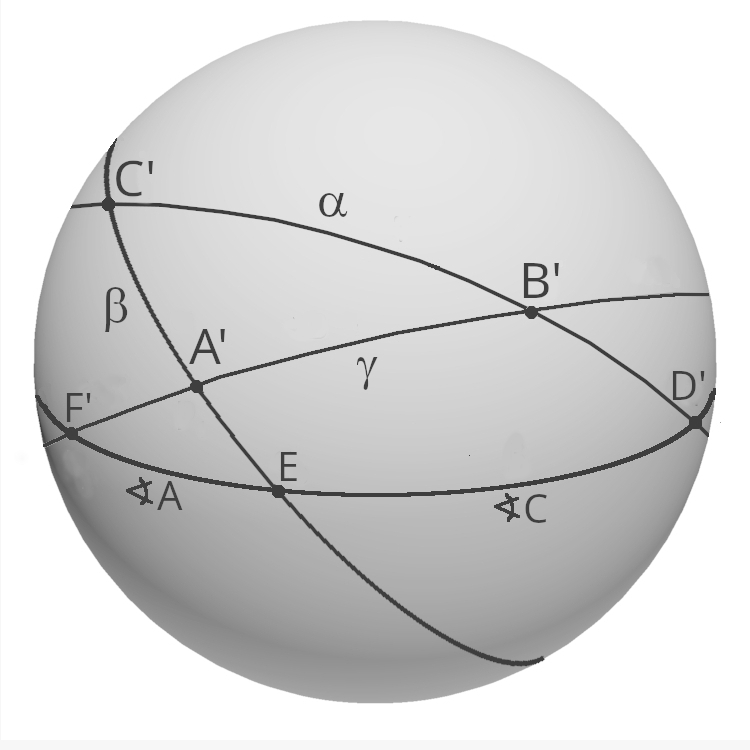
\includegraphics[width=6cm]{sphere2.jpg} \ }
\caption{Setup for the sphere-based rules} 
\end{figure} 


Begin with an arbitrary tetrahedron $\Delta ABCP$. Consider a small sphere centered at $P$ such that the other vertices are outside this sphere. For the purposes of this proof only, rescale three-dimensional real space so as to make the sphere a unit sphere $\mathcal{S}$. The plane through $P$ that is parallel to the plane containing $\Delta ABC$ intersects $\mathcal{S}$ in a great circle $\mathcal{E}$. The three rays from $P$ that pass through $A$, $B$ or $C$, each intersect $\mathcal{S}$ in a unique point. Accordingly, call these points $A'$, $B'$ and $C'$. As points on $\mathcal{S}$, they are all on the same side of $\mathcal{E}$ (a hemisphere). 

Consider the great circle $\mathcal{C}_1$ that passes through $B'$ and $C'$, the great circle $\mathcal{C}_2$ that passes through $C'$ and $A'$, and the great circle $\mathcal{C}_3$ that passes through $A'$ and $B'$. Notice that the great circle distance (along $\mathcal{C}_1$) between $B'$ and $C'$ is $\alpha$, the great circle distance (along $\mathcal{C}_2$) between $C'$ and $A'$ is $\beta$, and the great circle distance (along $\mathcal{C}_3$) between $A'$ and $B'$ is $\gamma$. Notice too that $\mathcal{C}_1$ is on the plane containing $B$, $C$ and $P$. Similarly for $\mathcal{C}_2$ and $\mathcal{C}_3$.

$\mathcal{C}_1$ intersects $\mathcal{E}$ in two antipodal points. Following $\mathcal{C}_1$ from $B'$ to $C'$, and continuing until we reach $\mathcal{E}$, call this intersection point $D$. Similarly, following $\mathcal{C}_1$ from $C'$ to $B'$, and continuing until we reach $\mathcal{E}$, call this intersection point $D'$. So again, $D$ and $D'$ are antipodal points on the sphere. Also, the directed line segment from $D'$ to $D$ is parallel to the directed line segment from $B$ to $C$. (Both are in the plane $PBC$, and the plane containing $\mathcal{E}$ is parallel to the plane $ABC$.)

Similarly define points $E$ and $E'$, using $\mathcal{C}_2$, and $F$ and $F'$, using $\mathcal{C}_3$. It is then straightforward to check that great-circle distances between $D$ and $E'$,  between $E'$ and $F$,  between $F$ and $D'$,  between $D'$ and $E$, between $E$ and $F'$, and between $F'$ and $D$ are respectively, $\angle C$, $\angle A$, $\angle B$, $\angle C$, $\angle A$ and $\angle B$. See Figure 1. Since $A'$, $B'$ and $C'$ lie in the same hemisphere, they form the vertices of a proper spherical triangle, whose side lengths are $\alpha$, $\beta$ and $\gamma$. Item 1 in the theorem follows immediately from this fact. 

Now, $C'$. $D'$ and $E$ are also the vertices of a proper spherical triangle. Moreover, the side connecting $C'$ and $D'$ contains $B'$, and side connecting $C'$ and $E$ contains $A'$. Let $\alpha + \delta$ be the length of the side connecting $C'$ and $D'$, and let $\beta + \epsilon$ be the length of the side connecting $C'$ and $E$ ($\delta, \epsilon > 0$). The side connecting $D'$ and $E$ has length $\angle C$. So, $\alpha + \beta + \angle C < (\alpha+\delta) + (\beta+\epsilon) + \angle C < 2 \pi$. This proves the third inequality in Item 3, and the other two inequalities are similarly obtained. By considering two paths on the sphere connecting $D'$ and $E$, we easily obtain $\angle C < \gamma + \delta + \epsilon$. Therefore, $\alpha + \beta - \gamma < \alpha + \beta - (\angle C - \delta - \epsilon) = (\alpha + \delta) + (\beta + \epsilon) - \angle C < 2\pi - 2 \angle C = 2 (\angle A + \angle B)$. This and similar reasoning yields Item 2 in the theorem. 

\end{proof} 

\noindent Note that, in the proof, it is possible for $\angle C$ to be less than $\gamma$. Figure 1 shows an example where $\angle A < \alpha$. 

\section{The Danger Cylinder and its Companion Surface} 

Going forward, we will always assume that the triangle $\Delta ABC$ is acute. It has long been understood that a P3P solution point $P$ in space, with coordinates $(x,y,z)$, is a repeated solution point if and only if it is on the circular cylinder that includes the circumcircle of the control points triangle. This cylinder is traditionally refered to as the ``danger cylinder." Using our setup, it is the cylinder whose equation is $x^2+y^2 = 1$. 

It is beneficial to understand the answer to a more subtle geometric question, as follows. For fixed control points, a generic point $P$ in space, with coordinates $(x,y,z)$, is a solution point to the P3P Problem for unique parameter values, $\alpha$, $\beta$ and $\gamma \;$ (namely, $\alpha = \angle BPC$, $\beta = \angle CPA$ and $\gamma = \angle APB$ ). In this way, we might say that $P$ determines an ``instance" of the P3P Problem. 

\begin{figure} 
\centerline{ 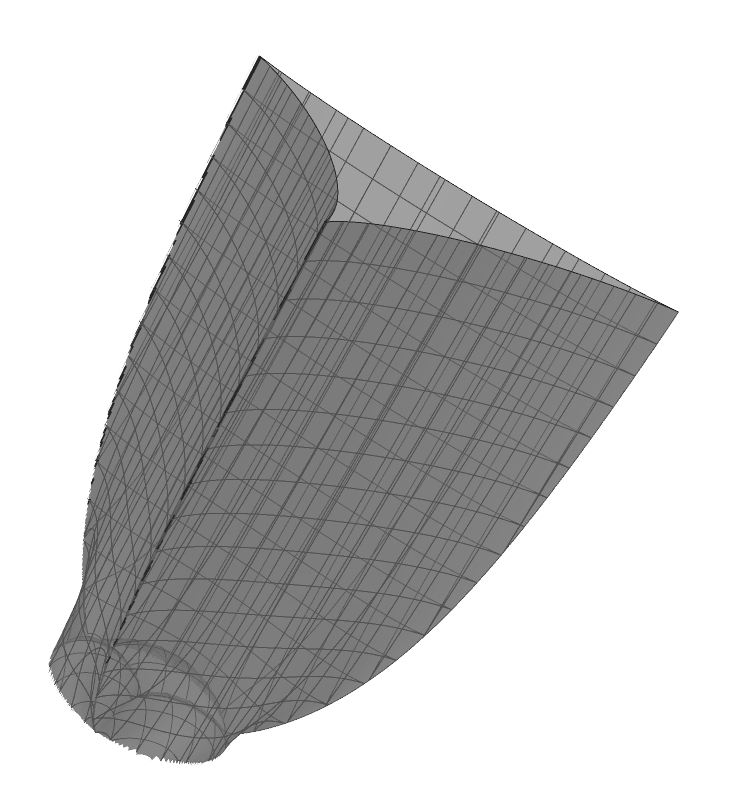
\includegraphics[width=6cm]{CSDC1.jpg} \ }
\caption{Companion surface to the danger cylinder} 
\end{figure} 

Assuming that $P$ is not on the danger cylinder, we now ask for a description of the surface that $P$ must lie on in order that its instance of the P3P Problem to have a repeated solution point (which will not be $P$). This surface was first described in \cite{R1}, and examined further in \cite{RW}, where it was given the name, ``the companion surface to the danger cylinder (CSDC)." Along with three double toroids, this surface plays an important role in partitioning space into various regions. Points in the same region have instances of the P3P Problem that have the same number of real solution points. 

Moreover, the region containing a point $P$ also determines which regions contain the other solution points for $P$'s instance of the P3P Problem. \cite{RW} deals with this in some detail, at least for the case where the control points triangle is acute. See Theorem 4 there. This is a rather complicated, but interesting, story, the essense of which will be largely reconstructed in this and the next sections of the current paper. 

Figure 2 shows what $CSDC$ looks like (for a typical acute control points triangle $\Delta ABC$) in the upper half space ($z > 0$). The lower half space ($z < 0$) portion is just the reflection of this about the $xy$-plane. In order to describe $CSDC$, a few results from \cite{RW} and \cite{R3} are now reproduced here, along with shorter proofs. For better motivated discussions of some of this material, consult these two documents. 

Following the practice used there, the $xy$-plane will here be identified with the complex plane by setting $\zeta = x + i \, y$. The control points / triangle vertices ($A$, $B$, $C$) are thus points $\zeta_j = x_j + i \, y_j$ in the complex plane with $| \zeta_j | = 1 \; (j = 1,2,3)$. Additionally, since $\phi_1+\phi_2+\phi_3 = 0$, we have $\zeta_1 \zeta_2 \zeta_3 = 1$. 

Let $Z=z^2$. Let $c_1 = \cos\alpha$, $c_2 = \cos\beta$ and $c_3 = \cos\gamma$. Let $D_1$, $D_2$ and $D_3$ denote the squared distances between control points, specifically, $D_1 = |\zeta_3-\zeta_2|^2$, $D_2 = |\zeta_1-\zeta_3|^2$, $D_3 = |\zeta_2-\zeta_1|^2$. It will also be useful to define $T_j = S_j \, - \, 2 \, D_j \, S_0 \, / \, (D_1+D_2+D_3) \; \; (j = 1,2,3)$, where $S_1$, $S_2$, $S_3$ and $S_0$ were defined in Section 1.
Three other quantities used in \cite{RW} and \cite{R3} will be needed here too: 
$$
\begin{array}{l} 
H \; = \; \eta^2 \; = \; T_1+ T_2+T_3 \; \; = \; \; S_1+S_2+S_2-2 S_0 \\ 
\quad \; \, =  1 - c_1^2 - c_2^2 - c_3^2 + 2 c_1 c_2 c_3 , \\
\zeta_H \, = \, x_H + i \, y_H \; = \; (x_1+x_2+x_3)+i(y_1+y_2+y_3),
\end{array}
$$
\noindent and $\zeta_L \; = $
$$
\begin{array}{l} 
\{ (\zeta_1^2+2\overline{\zeta_1}) T_1 + (\zeta_2^2+2\overline{\zeta_2}) T_2 + (\zeta_3^2+2\overline{\zeta_3}) T_3 \} \, / \, H.
\end{array}
$$

A cubic polynomial that has quite a useful role, expressed in terms of a complex indeterminate $\tau$, is the following: 
$$p(\tau) = \tau^3 - \zeta_L \tau^2 + \overline{\zeta_L} \tau - 1.$$ 

\vspace{2mm}

\begin{lemma}
The discriminant of the polynomial $p(\tau)$ is $\mathcal{D} \; \defeq \; \zeta_L^2 \, \overline{\zeta_L}^2 - 4 \, (\zeta_L^3 + \overline{\zeta_L}^3) + 18 \, \zeta_L \, \overline{\zeta_L} - 27$. Moreover, this quantity vanishes if and only if the P3P problem has a repeated solution for the specified parameters. 
\end{lemma}

\begin{proof}
The proposed formula for the discriminant is easily verified using the formula for the discriminant of a general cubic polynomial. In his solution to the P3P Problem, S. Finsterwalder introduced a certain cubic polynomial; see Equation (14) of \cite{HLON}. It is known that Grunert's system of equations has a repeated solution if and only if Finsterwalder's cubic polynomial has a repeated root. This of course is so if and only if the discriminant of this polynomial is zero. 

It will now be shown that Finsterwalder's cubic polynomial can be transformed via a M\"obius transformation (with constant coefficients) into the polynomial $p(\tau)$ times a nonzero constant, and vice-versa. This will establish that the discriminant of Finsterwalder's cubic polynomial is a nonzero constant multiple of the discriminant of $p(\tau)$. 

The M\"obius transformation is simply this:
$$\lambda \; = \; \frac{\zeta_1 (\zeta_3-\zeta_2)}{\zeta_3 (\zeta_2-\zeta_1)} \cdot \frac{\zeta_3 \, \tau - 1}{\zeta_1 \, \tau - 1} ,$$ 
and hence 
$$\tau \; = \; \frac{1}{\zeta_1 \zeta_3} \cdot \frac{\zeta_3 (\zeta_1-\zeta_2) \, \lambda - \zeta_1 (\zeta_2-\zeta_3)}{ (\zeta_1-\zeta_2) \, \lambda - (\zeta_2-\zeta_3)} .$$ 

Now, Finsterwalder's cubic polynomial is 
$$\mathcal{G} \, \lambda^3 + \mathcal{H} \, \lambda^2 + \mathcal{I} \, \lambda + \mathcal{J}$$
with $\mathcal{G} = D_3 (D_3 T_2 - D_2 T_3)$, $\mathcal{H} = D_2 (D_2-D_1) T_3 + D_3(D_3+2 D_1) T_2$, $\mathcal{I} = D_2 (D_2-D_3) T_1 + D_1(D_1+2 D_3) T_2$ and $\mathcal{J} = D_1 (D_1 T_2 - D_2 T_1)$. Upon substituting the formula for $\lambda$ in terms of $\tau$, and making other evident substitutions such as $D_1 = (\zeta_3-\zeta_2) (\overline{\zeta_3}-\overline{\zeta_2})$, etc., $\overline{\zeta_j} = 1 / \zeta_j \, (j = 1,2,3)$ and $\zeta_1 = 1 / (\zeta_2 \zeta_3)$, it is straightforward (though a bit tedious) to transform Finsterwalder's polynomial to $p(\tau)$ times a nonzero constant. 
\end{proof}

\noindent Further reasoning and motivation for the M\"obius transformation is provided in \cite{R3}. 

\vspace{2mm}

\begin{lemma}\footnote{This is Theorem 1 \cite{RW}.} 
For a given point $P$ in space, with coordinates $(x,y,z)$, consider the associated instance of the P3P problem (for which $P$ is a solution point). Then, 
$$\zeta_L \; = \; \zeta^2 \, - \, 2 \overline{\zeta} \, + \, ( \zeta \overline{\zeta} - 1 ) ( \zeta^2 - \zeta_H \zeta - \overline{\zeta} + \overline{\zeta_H}) \, / \, Z.$$
\end{lemma}

\vspace{2mm} 

\begin{proof}
Let $\zeta'_L$ denote the right side of the equation in the lemma; and so, we need to prove that $\zeta'_L$ = $\zeta_L$.
Let the $p(\tau)$ be as before, and let 
$$q(\tau) = \tau^3 - \zeta'_L \tau^2 + \overline{\zeta'_L} \tau - 1.$$ 
It suffices to show that the two cubic polynomials $p(\tau)$ and $q(\tau)$ are equal. To accomplish this, it will be shown that $p(\overline{\zeta_j}) = q(\overline{\zeta_j}) \; (j=1,2,3)$. Clearly $p(0) = q(0) = -1$. Then, the fact that the two cubic polynomials agree for four different values of the argument $\tau$ will imply that these polynomials are actually the same. The equation $(D_3 T_2 - D_2 T_3) / H = \zeta_1 p(\overline{\zeta_1}) / (\zeta_2-\zeta_3)$ can be checked directly by expanding each side to show that they have a common expression in terms of $\zeta_1$, $\zeta_2$, $\zeta_3$, $T_1$, $T_2$ and $T_3$. 

Because its circumradius is one, the square of the area of the control points triangle $\Delta ABC$ is $D_1 D_2 D_3 / 16$, and so the square of the volume of the tetrahedron having this triangle as a face, and the point $P$ as its opposite vertex, is $D_1 D_2 D_3 \, Z \, / \, 144$. The parallelepiped having the segments $\overline{PA}$, $\overline{PB}$ and $\overline{PC}$ as edges thus has squared volume $D_1 D_2 D_3 \, Z \,  / \, 4$. However, this must also equal the square of the Gramian determinant associated the vectors $\overrightarrow{PA}$, $\overrightarrow{PB}$ and $\overrightarrow{PC}$, which equals $H R_1 R_2 R_3$, where $R_1 = (\zeta - \zeta_1)(\overline{\zeta} - \overline{\zeta_1}) + Z$ is the squared distance between $P$ and $A$, etc. Therefore, $H = D_1 D_2 D_3 \, Z \, / \, (4 R_1 R_2 R_3)$. 

The Law of Cosines implies that $S_1 = 1 - c_1^2 = 1 - (R_2+R_3-D_1)^2 / (4 R_2 R_3) = (2 R_2 R_3 + 2 D_1 R_2 + 2 D_1 R_3 - D_1^2 - R_2^2 - R_3^2) / (4 R_2 R_3)$, and similarly for $S_2$ and $S_3$. Now, $(D_3 T_2 - D_2 T_3) / H =  (D_3 S_2 - D_2 S_3) / H =  4 R_1 R_2 R_3 (D_3 S_2 - D_2 S_3) / (D_1 D_2 D_3 \, Z)$, which can now be expanded and shown to equal $\zeta_1 q(\overline{\zeta_1}) / (\zeta_2-\zeta_3)$. It follows that $p(\overline{\zeta_1}) = q(\overline{\zeta_1})$. By symmetry, $p(\overline{\zeta_2}) = q(\overline{\zeta_2})$ and $p(\overline{\zeta_3}) = q(\overline{\zeta_3})$. 
\end{proof}

\vspace{2mm}

\begin{lemma}\footnote{This is part of Lemma 4 in \cite{RW}}
When the right side of the equation in Lemma 2 is substituted for $\zeta_L$, and likewise for $\overline{\zeta_L}$, into the formula for the discriminant $\mathcal{D}$ of $p(\tau)$, the result is $Z^{-4} \, (\zeta \overline{\zeta} - 1)^2 \, \mathcal{P}(\zeta, \overline{\zeta}, Z)$, where $\mathcal{P}(\zeta, \overline{\zeta}, Z)$ is a polynomial in $\zeta$, $\overline{\zeta}$ and $Z$. As a polynomial in $Z$ (with coefficients being polynomials in $\zeta$ and $\overline{\zeta}$), it has degree four. 

\end{lemma}

\begin{proof}
Let $D \; = \; Z^4 \, \mathcal{D} \; =$  
$$Z_L^2 \, \overline{Z_L}^2 - 4 \, Z \, (Z_L^3 + \overline{Z_L}^3) + 18 \, Z^2 \, Z_L \, \overline{Z_L} - 27 \, Z^4,$$
where $Z_L = Z \, \zeta_L$ , $\overline{Z_L} = Z \, \overline{\zeta_L}$ , and $Z$ is regarded as a real variable. Thus, $Z_L$, $\overline{Z_L}$ and $D$ can be expressed as polynomials in $\zeta$, $\overline{\zeta}$ and $Z$. As a polynomial in $Z$, $D$ has degree 4. 

If we momentarily set $\overline{\zeta} = 1 / \zeta$, we find that $Z_L = Z (\zeta^3 - 2) / \zeta$, and $\overline{Z_L} = Z (1 - 2 \zeta^3) / \zeta^2$, resulting in $D = 0$. Therefore, $\zeta \overline{\zeta} - 1$ is a factor of $D$ (no longer using the assumption that $\overline{\zeta} = 1 / \zeta$). 

Now, following common practice in complex analysis, treat $Z_L$ and $\overline{Z_L}$ as functions in independent variable $\zeta$, $\overline{\zeta}$ and $Z$. (A new variable could be substituted for $\overline{\zeta}$ here if desired.) Likewise, treat $D$ as a function in independent variables $Z_L$, $\overline{Z_L}$ and $Z$. Direct computations show that 
$$\left. \frac{\partial Z_L}{\partial \zeta} \right|_{\overline{\zeta}=1/\zeta} = \frac{ (1+2Z)\zeta^3 - \zeta_H \zeta^2 + \overline{\zeta_H}\zeta - 1}  {\zeta^2} , $$ 
$$\left. \frac{\partial \overline{Z_L}}{\partial \zeta} \right|_{\overline{\zeta}=1/\zeta} = \frac{-(1+2Z)\zeta^3 + \zeta_H \zeta^2 - \overline{\zeta_H}\zeta + 1}  {\zeta^3} , $$ 
$$\left. \frac{\partial D}{\partial Z_L} \right|_{\overline{\zeta}=1/\zeta} = \frac{-4 Z^3 (1+\zeta^3)^3}  {\zeta^5} , $$ 
and
$$\left. \frac{\partial D}{\partial \overline{Z_L}} \right|_{\overline{\zeta}=1/\zeta} = \frac{-4 Z^3 (1+\zeta^3)^3}  {\zeta^4}. $$
If we now regard $D$ as a function of $\zeta$, $\overline{\zeta}$ and $Z$, we obtain, by the chain rule, 
$$\left. \frac{\partial D}{\partial \zeta} \right|_{\overline{\zeta}=1/\zeta} \, = \, 0.$$ 
By symmetry, 
$$\left. \frac{\partial D}{\partial \overline{\zeta}} \right|_{\overline{\zeta}=1/\zeta} \, = \, 0.$$ 
It follows that $(\zeta \overline{\zeta} - 1)^2$ is a factor of $D$. 
\end{proof} 

\vspace{2mm}

$CSDC$ is simply defined to be the surface in ($xyz-$) space consisting of the points for which $\mathcal{P}(\zeta, \overline{\zeta}, Z) = 0$. Together with the danger cylinder ($\zeta \overline{\zeta} = 1$), we obtain all of the points for which the discriminant $\mathcal{D}$ of $p(\tau)$ vanishes. These are the points whose instance of the P3P Problem has a repeated solution. 

\vspace{2mm}

\begin{lemma}

$CSDC$ is unbounded, and as $Z\rightarrow \infty$, the orthogonal projection of $CSDC$ onto the $xy$-plane approaches the standard deltoid curve.  

\end{lemma}

\begin{proof}

By Lemma 2, as $Z \rightarrow \infty$, we see that $\zeta_L \rightarrow \zeta^2 \, - \, 2 \overline{\zeta}$, and so $\mathcal{D} \rightarrow$ 
$$(\zeta \overline{\zeta} - 1)^2 \; [ \, \zeta^2 \overline{\zeta}^2 - 4 (\zeta^3 + \overline{\zeta}^3) + 18 \zeta \overline{\zeta} - 27 \, ].$$
Thus, in the limit, $\mathcal{D}$ vanishes when $\zeta$ is on the unit circle and when $\zeta$ is on the standard deltoid curve, and nowhere else. The unit circle is expained by the fact that $\mathcal{D}$ vanishes on the danger cylinder. The standard deltoid curve must likewise by explained by the vanishing of $\mathcal{D}$ on $CSDC$, from which the claim in the lemma now follows. 

\end{proof}

\vspace{2mm}

\begin{lemma}

$CSDC$ consists of two surfaces $CSDC_0$ and $CSDC_1$, each symmetric about the $xy$-plane. Their intersection is the circumcircle of the triangle $\Delta ABC$. $CSDC_0$ is unbounded, and except for the circumcircle and three vertical lines on $DC$, $CSDC_0$ lies outside $DC$. Also, except for the circumcircle, $CSDC_1$ is inside the unit sphere, and hence bounded and inside $DC$. \\ 

\end{lemma} 

\begin{proof}

$CSDC$ is an algebraic surface, given by the polynomial equation $\mathcal{P}(\zeta, \overline{\zeta}, Z) = 0$. While $x^2+y^2-1$ is not a factor of this polynomial, it is a factor (in fact, a double factor) of the polynomial that results from setting $Z$ equal to zero. Thus, the circumcircle is part of $CSDC$. In fact the intersection of $CSDC$ and $DC$ consists of this circle and three vertical lines, namely, the lines where $\zeta = -1$ or $- e^{\pm 2\pi i/3}$. This can all be seen using the formula for $\mathcal{P}(\zeta, \overline{\zeta}, Z)$ in Lemma 16 of \cite{RW}. 

By Theorem 3 of \cite{RW}, the portion of $CSDC$ that is inside $DC$ is also inside the unit sphere, and hence is bounded. This is $CSDC_1$. By Lemma 4, we infer that $CSDC_0$ is unbounded, and that for $Z >> 0$, it asymptotically approaches the standard deltoid curve. So $CSDC_0$ is unbounded.   

\end{proof} 

\vspace{2mm}

When two points in space have the same values for $\alpha$, $\beta$ and $\gamma$, and hence solve the same instance of the P3P Problem, we will say that they are ``strongly related." When two points are either strongly related, or else have the same value for one of $\alpha$, $\beta$ or $\gamma$, and supplementary values for the other two, we will say that they are ``weakly related." Notice that two points are weakly related if and only if they have the same values for $c_1^2$,  $c_2^2$,  $c_3^2$ and $c_1 c_2 c_3$. ``Strongly related" and ``weakly related" are important equivalence relations. The significance of ``strongly related" for the P3P Problem is self-evident. The importance of ``weakly related" for the P3P Problem is made apparent in Lemma 6 (the next claim) and Lemma 7 (in the next section). 

\vspace{2mm}

\begin{lemma}

Let $P$ be a point in the upper half-space. 

\begin{enumerate} 

\item The reflection of $P$ about the $xy$-plane, in the lower half-space, is strongly related to $P$. 

\item If $P$ satisfies $D > 0$, then there exists exactly one other point in the upper-half space that is weakly related to it. 

\item If instead, $D < 0$, then there are exactly three such points in the upper-half space that are weakly related to $P$ (and to each other). 

\item If instead, $P$ is on $DC$, then, generally, there are exactly two other points in the upper half-space that are weakly related to it (and to each other), and these are on $CSDC$. This is so, except when $P$ is on the circumcircle of $\Delta ABC$ or on one of the three special vertical lines mentioned in Lemma 5, {\it i.e.}, when $P$ is on $DC \cap CSDC$.

\end{enumerate} 

\end{lemma} 

\begin{proof}

Item 1 is immediately clear from the symmetry of the P3P Problem about the $xy$-plane. Items 2 and 3 are just a restatement of Theorem 2 in \cite{RW}, which is proved there and will simply be assumed here. 

For Item 4, recall that a generic point on $DC$ serves as a double point for its instance of the P3P system of equations. This means that infinitesimally small perturbations of the P3P parameters $\alpha$, $\beta$ and $\gamma$ that causes $\mathcal{D}$ to be (infinitesimally) negative, would result in a P3P system with two distinct (real) solution points that are infinitesimally close to the original point. These two points are strongly related, and must be weakly related to two other points in the upper half-space. These latter two points must be infinitesimally close to two points on $CSDC$ since $\mathcal{D}$ is infinitesimally small. Therefore, by continuity, the original, unperturbed system must have two solution points on $CSDC$. However, if $P$ is on both $DC$ and $CSDC$, then there will be fewer than two other (distinct) points in the upper half-space that are weakly related to $P$.

\end{proof}

The last two lemmas in this section will be used in the next section to prove Theorem 2. Note too that the quantity $D$ defined in this section is the same as the $D$ defined in Section 1. To see this, one must expand using the definitions given in both sections. 


\section{The Deltoid-based Rules}

Before beginning a proof of Theorem 2, it is necessary to relay some more of the terminology, notation and results in \cite{RW}. While $A$, $B$ and $C$ will remain fixed, the point $P$ will move around in space continuously, and as such, will be called a ``particle," instead of a point. $P$ will thus trace out a continuous curve. Its movement can be regarded mathematically as a continuous map from an interval into 3-space, thereby supplying mathematical rigor. However, to gain better intuition of the analysis, thinking about $P$ moving dynamically is quite helpful. Fixed points can be regarded as stationary particles. 

The plan for proving Theorem 2 is to show that certain possible regions of space, designated below as $110^+, 101^+, 011^+$ and $111^+$, actually do not exist. Lemmas 14 and 15 establish this claim, after which the proof of Theorem 2 quickly follows.

As a particle $P$ moves, its values of $\alpha$, $\beta$, $\gamma$, $c_1$, $c_2$ and $c_3$ will change continuously, usually. However, it will sometimes be necessary to allow $P$ (or another particle) to pass through a control point ($A$, $B$ or $C$). At the momemt when this occurs, two of the angles ($\alpha$, $\beta$, $\gamma$) and two of the cosines ($c_1$, $c_2$, $c_3$) will not be defined. As $P$ pass through the control point, the signs of these two cosines will instantaneously change, because the corresponding angles will instantaneously be replaced with their supplementary angles. 

The toroid $\mathcal{T}_A$ consists of all the points in space for which $\alpha = A$. This is the surface obtained by taking the open arc on the circumcircle of $\Delta ABC$ that connects $B$ and $C$, and that passing through $A$, and rotating it about the line through $B$ and $C$. Note that we are deliberatly excluding the points $B$ and $C$ from $\mathcal{T}_A$. Using the coordinate system from Section 1, this circumcircle is simply the unit circle in the $xy$-plane. Apart from the arc that we started with, the toroid $\mathcal{T}_A$ stays outside the unit sphere. Let $\overline{\mathcal{T}}_A = \mathcal{T}_A \cup \{B,C\}$, which will also be called a toroid.

If we instead start with the open arc on the circumcircle connecting $B$ and $C$ that does not pass through $A$, and again rotate about the line through $B$ and $C$, then we obtain a different, but related, toroid, which will be denoted $\mathcal{T}_{\pi-A}$. This is the surface on which $\alpha = \pi - A$. Apart from the starting arc, this toroid stays inside the unit sphere and hence inside $\overline{\mathcal{T}}_A$. Let $\overline{\mathcal{T}}_{\pi-A} = \mathcal{T}_{\pi-A} \cup \{B,C\}$, which will also be called a toroid. The toroids $\mathcal{T}_B, \mathcal{T}_{\pi-B}, \mathcal{T}_C, \mathcal{T}_{\pi-C}, \overline{\mathcal{T}}_B, \overline{\mathcal{T}}_{\pi-B},\overline{\mathcal{T}}_C$ and $\overline{\mathcal{T}}_{\pi-C}$ are similarly defined. All of these toroids will be refered to as ``basic toroids."

Consider three-dimensional real space with these toroids removed: $\overline{\mathcal{T}}_A, \overline{\mathcal{T}}_{\pi-A}, \overline{\mathcal{T}}_B, \overline{\mathcal{T}}_{\pi-B}, \overline{\mathcal{T}}_C$ and $\overline{\mathcal{T}}_{\pi-C}$. The connected components of the resulting space will be called ``toroidal regions." Each is identified by means of a three-digit code, where the first digit relates to the toroids $\overline{\mathcal{T}}_A$ and $\overline{\mathcal{T}}_{\pi-A}$, the second digit relates to the toroids $\overline{\mathcal{T}}_B$ and $\overline{\mathcal{T}}_{\pi-B}$, and the third digit relates to the toroids $\overline{\mathcal{T}}_C$ and $\overline{\mathcal{T}}_{\pi-C}$. If the first digit is 0, then the region is outside $\overline{\mathcal{T}}_A$; if it is 1, then the region is between $\overline{\mathcal{T}}_A$ and $\overline{\mathcal{T}}_{\pi-A}$; and if it is 2, then the region is inside $\overline{\mathcal{T}}_{\pi-A}$. Similarly for the second and third digits. For example, 001 refers to the region outside $\overline{\mathcal{T}}_A$ and $\overline{\mathcal{T}}_B$, but inside $\overline{\mathcal{T}}_C$.

Notice that the identification code for a toroidal region cannot involve a 0 and a 2, since that would suggest that there are points that are both outside and inside the unit sphere. Also, 222 is not a valid identification code, since no point can be inside $\overline{\mathcal{T}}_{\pi-A}$, inside $\overline{\mathcal{T}}_{\pi-B}$, and inside $\overline{\mathcal{T}}_{\pi-C}$. (These three toroids intersect in a single point, namely, the orthocenter of $\Delta ABC$.) Notice too, that when the first digit of an identification code is 0, this means that $\alpha < \angle A$; when it is 1, this means that $\angle A < \alpha < \pi-\angle A$; when it is 2, this means that $\alpha > \pi - \angle A$. Similarly for the other two digits.  

\begin{figure} 
\centerline{ 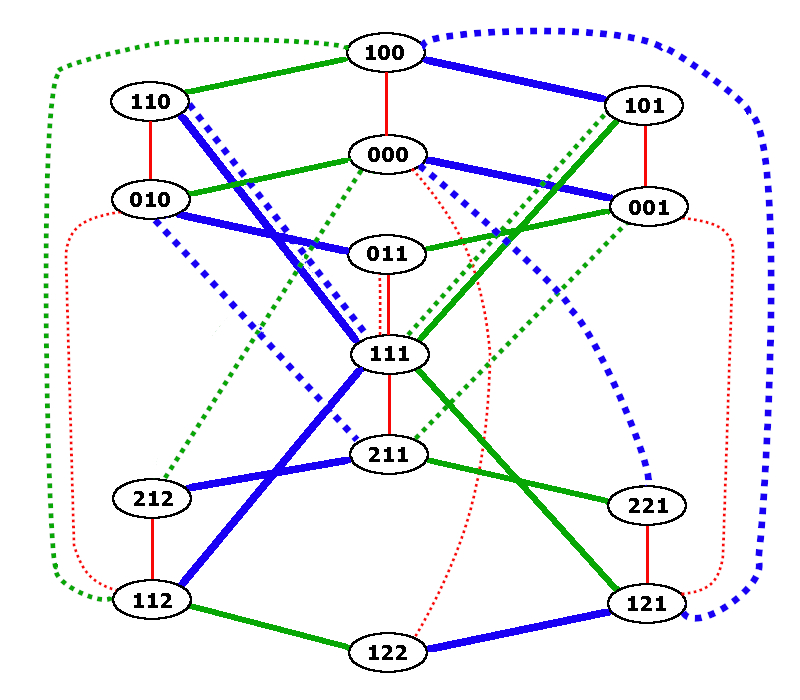
\includegraphics[width=7cm]{RegionsGraph_0.jpg} \ }
\caption{Transition graph for toroidal regions} 
\end{figure} 

Figure 3 is reproduced from \cite{RW}. It shows a graph that indicates how it is possible for a particle to continuously transition from one toroidal region to another, either by passing through one of the above toroids (solid edges in the graph) or by passing through one of the control points (dotted edges in the graph). The thickness/color of a solid edge indicates which toroid the particle passes through: thin/red for $\mathcal{T}_A$ or $\mathcal{T}_{\pi-A}$, medium/green for $\mathcal{T}_B$ or $\mathcal{T}_{\pi-B}$, and thick/blue for $\mathcal{T}_C$ or $\mathcal{T}_{\pi-C}$. Similarly the thickness/color of a dotted edge indicates which control point the particle passes through. 

For example, the solid edge connecting 121 and 122 represents moving across $\mathcal{T}_{\pi-C}$, while staying inside $\mathcal{T}_{\pi-B}$, and between $\mathcal{T}_{\pi-A}$ and $\mathcal{T}_A$. The dotted edge connecting 100 and 121 represents passing through vertex $C$ and thereby changing toroidal regions as follows. If the particle begins between $\mathcal{T}_{\pi-A}$ and $\mathcal{T}_A$, but outside $\mathcal{T}_B$ and $\mathcal{T}_C$, it will stay between $\mathcal{T}_{\pi-A}$ and $\mathcal{T}_A$, but it will move inside $\mathcal{T}_{\pi-B}$, and be between $\mathcal{T}_{\pi-C}$ and $\mathcal{T}_C$. This can be visualized by considering one double toroid at a time, such as $\mathcal{T}_{\pi-A} \cup \mathcal{T}_A$, and zooming in on vertex $C$. In doing so, each of $\mathcal{T}_{\pi-A} \cup \mathcal{T}_A$ and $\mathcal{T}_{\pi-B} \cup \mathcal{T}_B$ is approximated by a double cone with apex $C$, while $\mathcal{T}_C$ is approximated by a plane, and $\mathcal{T}_{\pi-C}$ simply vanishes, since $C$ is outside $\overline{\mathcal{T}_{\pi-C}}$. 

It will be helpful to subdivide the toroidal regions into smaller regions by cutting them with the surface $DC \cup CSDC$ (where $D = 0$). Let $000^+$ amd $000^-$ denote the portions of toroidal region $000$ where $D > 0$ and where $D < 0$, respectively. And so forth. A goal now is to show that regions $011^+$, $101^+$, $110^+$ and $111^+$ do not exist. This will establish that Rules 6 and 7 in Conjecture 1 are necessary conditions, that is, it will prove Theorem 2. A series of lemmas will ultimately lead to this objective. 


As we move a particle $P$ around in space, we consider all of the other possible particles that would stay weakly related to $P$. The next result gives a sense of how these particles would behave. 

\vspace{2mm}

\begin{lemma}

When a particle $P$ passes (generically) through $\mathcal{T}_A$ or $\mathcal{T}_{\pi-A}$, exactly one of the other particles weakly related to it, in the upper half-space, and its reflection in the lower half-space (also weakly related to $P$), will pass through the vertex $A$. As it does, its values of $c_2$ and $c_3$ will instantaneously be negated because its values of the $\beta$ and $\gamma$ angles will instantaneously be replaced by their supplements. The particles will remain weakly related to $P$ (and each other) after one of them passes through $A$. Of course, what has been said here concerning $\mathcal{T}_A$ and $\mathcal{T}_{\pi-A}$ applies in a symmetrical manner to $\mathcal{T}_B$, $\mathcal{T}_{\pi-B}$, $\mathcal{T}_C$ and $\mathcal{T}_{\pi-C}$. 

\end{lemma}

\begin{proof}

Lemma 9 in \cite{RW} immediately implies all that is said here concerning $P$ passing through $\mathcal{T}_A$. A small adjustment in the reasoning in the proof of Lemma 9 in \cite{RW} likewise handles the case when $P$ passes through $\mathcal{T}_{\pi-A}$ instead. In both cases, the reasoning begins as follows. Consider the three lines that pass through $P$ and one of the control points, when $P$ is on $\mathcal{T}_A$ or on $\mathcal{T}_{\pi-A}$. This configuration of lines can be rigidly moved so as to now intersect at $A$ and still pass through the control points. 

\end{proof}

Note that at the exact moment that when the particle passes through one of the control points, two of the angles $\alpha$, $\beta$, $\gamma$ will be undefined, and so the notions of ``strongly related" and ``weakly related" break down momentarily. However the algebraic geometric technique of ``blowing up" the control points can correct this deficiency for the weak relationship, but not the strong relationship. As the particle passes through the control point, its weak relationships with other particles continues unimpeded; not so for its strong relationships with other particles. ``Weakly related" is an important equivalence relation for achieving a better understanding of the nature of the P3P problem, since it is maintained under continuous motion, even when passing through a control point.

A scenerio that will be of particular interest in this paper, but which was not considered in the other papers, is this: Assume that a particle $P$ starts off on $DC$, high above the $xy$-plane ($z \gg 0$). Suppose that $P$ moves along a vertical line on $DC$ until it reaches the circumcircle of $\Delta ABC$. Let us say that $\phi$ is a fixed angle such that this line is describe by $(x, y) = (\cos\phi, \sin\phi)$. 

A description of this scenario begins by asking whether or not this line intersects one of the basic toroids. It will be helpful to let $\phi_1'$ be either $(\phi_2 + \phi_3)/2$ or $\pi + (\phi_2 + \phi_3)/2$, such that the point $(\cos \phi_1', \sin \phi_1')$ lies midway between $B$ and $C$ along the arc of the circumcircle connecting $B$ and $C$ that does not contain $A$ (the shorter arc connecting $B$ and $C$). Similarly for $\phi_2'$ and $\phi_3'$. 

\vspace{2mm}

\begin{lemma}
 
The vertical line on $DC$, described by $(x, y) = (\cos\phi, \sin\phi)$ for fixed $\phi$, intersects the toroid $\overline{\mathcal{T}}_A$ in the upper half-space ({\it i.e.} $z > 0$) if and only if $\phi_1' - \pi/2 < \phi < \phi_1' + \pi/2$ \ (mod $2\pi$), that is, if and only if there exists an integer $k$ such that $\phi_1' - \pi/2 < \phi - 2k\pi < \phi_1' + \pi/2$.

\end{lemma}

\begin{proof}

The equation for the double toroid $\mathcal{T}_A \, \cup \, \mathcal{T}_{\pi-A}$ can be obtained from $c_1^2 = \cos^2 \angle A$. Lemma 7 of \cite{RW} works this out to be the following:

\vspace{-2mm} 

$$\begin{array}{l} 
Z^2 + [ \, 2 \, \zeta \, \overline{\zeta} - (\overline{\zeta_2} + \overline{\zeta_3}) \, \zeta  - (\zeta_2 + \zeta_3) \, \overline{\zeta} - 2 \, ] \, Z \\
+ \; ( \zeta \overline{\zeta} - 1) \, [ \; \zeta \, \overline{\zeta} - (\overline{\zeta_2} + \overline{\zeta_3}) \, \zeta  - (\zeta_2 + \zeta_3) \, \overline{\zeta} \\
+ \; (1 + \zeta_2 \overline{\zeta_3} + \overline{\zeta_2} \zeta_2 ) \; ] \; = \; 0. 
\end{array}$$

\vspace{2mm} 

Again $Z=z^2$. Consider the intersection of this double toroid with the danger cylinder. $DC$ is given by the equation $\zeta \overline{\zeta} = 1$. Substituting $1/\zeta$ for $\overline{\zeta}$ in the formula for the double toroid yields 

$$Z \; = \; \frac{(\overline{\zeta_2} \, + \, \overline{\zeta_3}) \, \zeta^2 + (\zeta_2 + \zeta_3)} {\zeta} {\ \atop ,} $$ 

\vspace{2mm} 

\noindent provided that $\zeta$ is nonzero. The curve described by this equation, let us call it $\Gamma$, intersects the $xy$-plane at the two points given by 

$$ \zeta^2 \; = \; - \, \frac{\zeta_2 + \zeta_3}{\overline{\zeta_2} + \overline{\zeta_3}} \; = \; - \, \frac{(\zeta_2 + \zeta_3)^2}{|\zeta_2 + \zeta_3|^2} {\ \atop .} $$

\vspace{2mm}

\noindent The two points are therefore 

$$ \zeta \; = \; \pm i \; \frac{\zeta_2 + \zeta_3}{|\zeta_2 + \zeta_3|} {\ \atop .} $$

\vspace{2mm}

Now, setting $\zeta_1' = (\zeta_2 + \zeta_3) / |\zeta_2 + \zeta_3|$, we see that . 

\vspace{-4mm} 

$$ \frac{(\overline{\zeta_2} \, + \, \overline{\zeta_3}) \zeta_1'^2 + (\zeta_2 + \zeta_3)} {\zeta_1'} \; = \; 2 |\zeta_2+\zeta_3| \; > \; 0, $$ 

\vspace{2mm} 

\noindent We can then reason that the open semicircle portion of the unit circle in the $xy$-plane that connects the antipodal points $\pm i \, (\zeta_2 + \zeta_3) / |\zeta_2 + \zeta_3|$, and that has $\zeta_1'$ as its midpoint, is the vertical projection of $\Gamma$ onto the $xy$-plane. Moreover, letting $\zeta = \exp(i \phi)$ range over this semicircle, we see that $\phi$ ranges (modulo $2\pi$) over the values given in the lemma. 
 
\end{proof} 

\noindent Note that the unit circle in the $xy$-plane is also part of the intersection of $DC$ and the double toroid
$\overline{\mathcal{T}}_A \cup \overline{\mathcal{T}}_{\pi-A}$. Also, no part of $\overline{\mathcal{T}}_{\pi-A}$ not on this unit circle intersects $DC$. 

As $P$ moves along the vertical line on $DC$, we consider two other particles, $P'$ and $P''$, that stay weakly related to $P$, and so stay on $CSDC$ (by Lemma 6), and which also start off high above the $xy$-plane. They will initially move downward along $CSDC$, but the situation becomes more complicated as soon as $P$ crosses one of the three basic toroids. We need to track the movement of $P$, $P'$ and $P''$ as carefully as possible. 

Towards this goal, additional ideas and notation from \cite{RW} are needed here. Begin by observing that when $P$, $P'$ and $P''$ are all high about the $xy$-plane, they are all in toroidal region 000. Let us consider how this might change as $P$ descends along the verticle line. 

Notice that if $P$ goes into toroidal region 110, either by first going into 100 or 010, then $P'$ must either also move into  toroidal region 110 or move into toroidal region 112. If could, for instance, wind up in 112 by first crossing $\overline{\mathcal{T}}_A$ to arrive in 100, and then going through $B$ to arrive in 112. (See the discussion of Figure 3.)

However, even if we know that $P'$ is in region 110, it is initially unclear whether $P$ and $P'$ have the same values for $\alpha$ and $\beta$, or have supplementary values for these angles. Similarly, two possibilities seemingly exist if we know that $P'$ is in region 112 instead. To capture a sense of the possibilities, we will say that when $P$ is in toroidal region 110, the pair of particles $(P, P')$ will be in one of these four ``configurations:" $(110, 110)$, $(110, \underline{1}\,\underline{1}0)$, $(110, \underline{1}12)$, $(110, 1\underline{1}2)$. In writing, for instance, the configuration $(110, \underline{1}12)$, we are indicating that $P$ is in toroidal region 110, $P'$ is in toroidal region 112, and that these two particles have the same value for $\beta$, but supplementary values for $\alpha$, and supplementary values for $\gamma$. 

The ``$0$'' at the end of ``$110$" and the ``$2$" at the end of ``$\underline{1}12$" clearly indicate that the $\gamma$ values differ. The ``$1$" at the start of  ``$110$" and the ``$\underline{1}$" at the start of ``$\underline{1}12$" indicate that the $\alpha$ values differ. An underlined 1 suggests that the corresponding angle is the supplement of what it would be if the 1 was not underlined. The configuration $(110, \underline{1}12)$ is the same as the configuration $(\underline{1}10, 112)$. In other words, which of the two leading ones we underline is irrelevant.

The notation can be extended to discuss more than two particles. For instance, based on the discussion so far, it seems that $(P, P', P'')$ might have configuration $(110, \underline{1}\,\underline{1}0, \underline{1}12)$, at some moment. Theorem 2 will now be proved via a series of lemmas. 

\vspace{2mm}

\begin{lemma}

As $P$ descends down the line $(x, y) = (\cos\phi, \sin\phi)$, beginning with $z \gg 0$ and continuing until $z$ is arbitrarily close to, but not equal to, zero, it will pass through one or two of the basic toroids, $\mathcal{T}_A$, $\mathcal{T}_B$, $\mathcal{T}_C$, but never all three of them. 

\end{lemma}

\begin{proof}

The triangle vertices are $A \, (= \zeta_1)$, $B \, (= \zeta_2)$ and $C \, (= \zeta_3)$. With $\phi_1'$, $\phi_2'$ and $\phi_3'$, as defined earlier, let $A' = \zeta_1' = \exp( i \, \phi_1' )$, $B' = \zeta_2' = \exp( i \, \phi_2' )$ and $C' = \zeta_3' = \exp( i \, \phi_3' )$. Restricting movement to the unit circle, denote the (arc) distance between two points $\zeta$ and $\zeta'$ by $d(\zeta, \zeta')$. 

Lemma 8 gives the range of $\phi$ that would cause $P$ to pass through $\mathcal{T}_A$. This corresponds to an open semicircle ( $\zeta = \exp(i \phi)$ ) on the unit circle in the $xy$-plane. Call this semicircle $\sigma_A$. Similarly, let semicircles $\sigma_B$ and $\sigma_C$ correspond to $\mathcal{T}_B$ and $\mathcal{T}_C$, respectively. These three semicircles cannot all overlap, but must intersect pairwise. To see this, reason as follows. 

First, $\sigma_A$ cannot contain $A$ because the vertical line through $A$ clearly does not intersect $\mathcal{T}_A$ in the upper half-space. Of course, $\sigma_A$ does contain the point $A' = \exp(i \, \phi_1')$, which is in fact the midpoint of this semicircle (see Lemma 8). Likewise, $\sigma_B$ has $B'$ as its midpoint, but does not contain $B$, and $\sigma_C$ has $C'$ as its midpoint, but does not contain $C$. 

Now, $d(B, C) = 2 d(A', B) = 2 d(A', C) < \pi$. By this and symmetrical reasoning, we obtain $d(A', B) < \pi/2$, $d(A', C) < \pi/2$, $d(B', C) < \pi/2$, $d(B', A) < \pi/2$, $d(C', A) < \pi/2$ and $d(C', B) < \pi/2$. So, $d(B', C') < \pi$, $d(C', A') < \pi$ and $d(A', B') < \pi$. By the Inscribed Angle Theorem, we get $\angle C'A'B' < \pi/2$, $\angle A'B'C' < \pi/2$, $\angle C'B'A' < \pi/2$, That is, the triangle $\Delta A'B'C'$ is acute. 

Letting $O$ denote the origin, notice that $O$ is the circumcenter of both $\Delta ABC$ and $\Delta A'B'C'$.  Here are additional facts that are straightforward to check: $2 \angle AOC' = \angle AOB, \; 2 \angle AOB' = \angle AOC, \; \angle BOC = 2\pi - \angle AOB - \angle AOC = 2 (\pi - \angle AOC' - \angle AOB') = 2(\pi - \angle B'OC'$. So, $\angle B'OC' = \pi - \frac{1}{2} \angle BOC > \pi - \pi / 2 = \pi / 2$. Likewise, $\angle C'OA' > \pi / 2$ and $\angle A'OB' > \pi / 2$. It follows that $\sigma_A$ does not contain $B'$ nor $C'$, that $\sigma_B$ does not contain $C'$ nor $A'$, and that $\sigma_C$ does not contain $A'$ nor $B'$.

It is now straightforward to see that any two of $\sigma_A$, $\sigma_B$ and $\sigma_C$ overlap in an arc of length strictly between 0 and $\pi / 2$. From this, it is straightforward to argue that no point can be on all three of these semicircles. Also, every point on the unit circle (in the $xy$-plane) is within a (arc) distance $\pi / 2$ of at least one of $A'$, $B'$ and $C'$, and so is on at least one of the three semicircles.  

\end{proof}

\vspace{2mm}

\begin{lemma}

As $P$ descends from $z \gg 0$, as in Lemma 9, assume that the first of the basic toroids it crosses is $\mathcal{T}_A$. As it crosses, the configuration for $(P, P', P'')$ will change from $(000, 000, 000)$ to $(100, 100, 122)$ or $(100, 122, 100)$. Similarly if $P$ crosses first through $\mathcal{T}_B$ or $\mathcal{T}_C$, instead of $\mathcal{T}_A$.  \\

\end{lemma}

\begin{proof}

When $P$ crosses $\mathcal{T}_A$, it enters toroidal region 100. Because of Lemma 7, either $P'$ or $P''$, but not both, must pass through the vertex $A$. Upon doing so, it will enter toroidal region 122 because its values of $\beta$ and $\gamma$ will be instantaneously replaced by their supplementary angles, and because it will also have moved inside $\overline{\mathcal{T}}_A$. The remaining particle will simply cross $\mathcal{T}_A$ as $P$ crosses $\mathcal{T}_A$, and so also enter toroidal region 100.  

\end{proof}

\vspace{2mm}

\begin{lemma}

If $P$ moves as in Lemma 10, and if $P$ does not cross another basic toroid before reaching the $xy$-plane, whichever of $P'$ and $P''$ passed through the vertex $A$ will continue to move until it reaches the orthocenter $H$ of $\Delta ABC$. The remaining particle will move until it arrives at some point on the circumcircle (unit circle). In doing so, after $P$ passes through $\overline{\mathcal{T}}_A$, none of the three particles ($P$, $P'$, $P''$) will cross the surface $\overline{\mathcal{T}}_A \, \cup \, \overline{\mathcal{T}}_{\pi-A} \, \cup \, \overline{\mathcal{T}}_B \, \cup \, \overline{\mathcal{T}}_{\pi-B} \, \cup \, \overline{\mathcal{T}}_C \, \cup \, \overline{\mathcal{T}}_{\pi-C}$. \\ 

\end{lemma}

\begin{proof}

The points on the circumcircle, other than the vertices $A$, $B$ and $C$, are weakly related to each other. By the Inscribed Angle Theorem, while moving a particle around on the circumcircle, its $\alpha$, $\beta$ and $\gamma$ values remain constant until one of the three vertices is crossed. Upon crossing, two of these angles get replaced by their supplements, while the third is unaffected.  At each of the non-vertex points on the circumcircle, $(\alpha, \beta, \gamma)$ equals one of the following: $(\pi-\angle A, \angle B, \angle C)$, $(\angle A, \pi-\angle B, \angle C)$, $(\angle A, \angle B, \pi-\angle C)$.  

Now, the orthocenter $H$ of $\Delta ABC$ is weakly related to all of these non-vertex points on the circumcircle. Here $\alpha = \pi - A$, $\beta = \pi - B$, $\gamma = \pi - C$. Reasoning using continuity, it can be seen that as a particle moves in three dimensions, and as it approaches a non-vertex point on the circumcircle, staying above the $xy$-plane, one and only one of its weakly related particles above the $xy$-plane must approach $H$. The details for this argument are omitted here, but the reasoning involves the locally continuous and non-singular behavior of each of the quantities $\alpha$, $\beta$ and $\gamma$. 

Returning to the setup in the lemma, one of $P'$ and $P''$ must therefore approach $H$ as $P$ approaches a non-vertex point on the circumcircle. The other has no place to go to other than a different non-vertex point on the circumcircle. Moreover, after $P$ passes through $\overline{\mathcal{T}}_A$, since it never crosses $\overline{\mathcal{T}}_A \, \cup \, \overline{\mathcal{T}}_{\pi-A} \, \cup \, \overline{\mathcal{T}}_B \, \cup \, \overline{\mathcal{T}}_{\pi-B} \, \cup \, \overline{\mathcal{T}}_C \, \cup \, \overline{\mathcal{T}}_{\pi-C}$ again, its weakly related particles $P'$ and $P''$ cannot (again) pass through this surface. Whichever of $P'$ and $P''$ went through $A$ is the only one that can reach the point $H$, which is inside $\Delta ABC$, under these restrictions.

\end{proof}

\vspace{2mm}

\begin{lemma}

Suppose that $P$, $P'$ and $P''$ moves as in Lemma 10, but that after $P$ crosses $\overline{\mathcal{T}}_A$, it next crosses $\overline{\mathcal{T}}_B$ before arriving on the circumcircle of $\Delta ABC$. Assuming that $P''$ goes through the vertex $A$, later, $P'$ will go through the vertex $B$. The configuration for $(P, P', P'')$ will change like so: 

\vspace{-2mm} 

$$(000, 000, 000) \rightarrow (100, 100, 122) \rightarrow (110, \underline{1}12, 1\underline{1}2). $$

\vspace{2mm} 

\noindent Similarly, if we permute the vertices and/or switch the roles of $P'$ and $P''$. 

\end{lemma}

\begin{proof}

The intermediate configuration is clear from Lemma 10 and its proof. Now, either $P'$ or $P''$ (but not both) must then go through $B$. However, $P''$ cannot go through $B$, because, at the moment when it would need to do so, it will be inside $\overline{\mathcal{T}}_{\pi-B}$, and so cannot reach $B$. So $P'$ must go through $B$. It is straightforward to then check that the final configuration must be as claimed. 

\end{proof}

\vspace{2mm}

\begin{lemma}

Consider two particles $P$ and $P'$ in the upper half-space which maintain a weak relationship with each other, and which keep $D > 0$. (In this case, no other particle in the upper half-space can be weakly related to these.) Then, $P$ and $P'$ cannot both be in toroidal region 110. Similarly for 101 and 011. \\ 

\end{lemma}

\begin{proof}

The region $110^+$ is outside the unit sphere since it is outside $\overline{\mathcal{T}}_C$. By Lemma 5, it is outside $CSDC_0$ too since $D > 0$ throughout the region. It is thus outside $DC$ too. It is also a bounded region since toroidal region 110 is bounded. Assume that $P$ are $P'$ are both in toroidal region $110^+$. Then, $(P, P')$ must be in one of these two configuration: $(110, 110)$ or $(110, \underline{1}\underline{1}0)$. 

First suppose the configuration is $(110, 110)$. Maintaining $D > 0$, suppose $P$ moves so as to pass through one of the basic toroids. $P$ cannot cross $\mathcal{T}_A$ because $P'$ cannot reach the vertex $A$. If it could, then, upon passing through it, the configuration would need to change to $(010, 0\underline{1}2)$, but there is no toroidal region 012. Similarly, $P$ cannot cross $\mathcal{T}_B$. The boundary of region $110^+$ must be a subset of $\overline{\mathcal{T}}_C \, \cup \, CSDC_0$. However, the region  $110^+$ is outside $\overline{\mathcal{T}}_C \, \cup \, CSDC_0$. Since $110^+$ is bounded, this is not possible. So the configuration $(110, 110)$ is not possible. 

Now consider the $(110, \underline{1}\underline{1}0)$ possibility. From here, $P$ cannot reach $\mathcal{T}_A$ since $P'$ cannot reach $A$ simultaneously. This is because when $P$ arrives at $\mathcal{T}_A$, its $\alpha$ will equal $\angle A$, so $P'$ will have $\alpha = \pi - \angle A$. However, $P'$ needs to have $\alpha = \angle A$ when it passes through $A$. Likewise, $P$ cannot reach $\mathcal{T}_B$. By the same reasoning as before, this leads to a contradiction. 
We must conclude that $(110, \underline{1}\underline{1}0)$ is impossible too. Consequently, $P$ and $P'$ cannot both be in toroidal region 110. Likewise, still assuming $D > 0$, they cannot both be in toroidal region 101 nor toroidal region 011.  

\end{proof}

\vspace{2mm}

\begin{lemma}

Consider again two particles $P$ and $P'$ in the upper half-space which maintain a weak relationship with each other, and which keeps $D > 0$. $P$ cannot be in toroidal region 110 while $P'$ is in toroidal region 112. Therefore, $D \le 0$ throughout toroidal region 110, and $D = 0$ can only happen for a point on $DC$. Ditto for toroidal regions 101 and 011. \\

\end{lemma}

\begin{proof}

Assume that $P$ is in toroidal region 110 and that $P'$ is in toroidal region 112. Then, $(P, P')$ must be in one of these two configuration: $(110, 1\underline{1}2)$ or $(110, \underline{1}12)$. By symmetrical reasoning, we may assume $(110, 1\underline{1}2)$. $P'$ cannot reach vertex $C$, so $P$ cannot reach $\mathcal{T}_C$. Also, $P'$ cannot reach vertex $B$ while $P$ arrives at $\mathcal{T}_B$, since $P$ and $P'$ have supplementary values for $\beta$, instead of equal values. 

Now, if $P$ goes through $\mathcal{T}_A$, and $P'$ goes through $A$, then the configuration will become $(010, 010)$. $P$ could not now pass through $\mathcal{T}_B$ because that would require $P'$ to pass through $B$, resulting in the configuration $(000, 202)$, which is impossible. Yet, $P$ should be able to reach $\mathcal{T}_B$ from inside region $010^+$ (the part of toroidal region 010 for which $D > 0$), resulting in a contradiction. This is because the boundary of 
any connected component of $010^+$ must include part of $\mathcal{T}_B$, since otherwise, this region will not be bounded. 

Thus, we see that $P$ cannot be in toroidal region 110 while $P'$ is in toroidal region 112. Since they cannot both be in toroidal region 110 (by Lemma 13), we must conclude that $P$ cannot be in toroidal region 110. That is, $D$ must be less than or equal to zero throughout toroidal region 110. However, Lemmas 10 and 12 make equality impossible unless the point is on $DC$. Those lemmas capture a complete sense of where a particle for which $D = 0$ can be. Such a particle is on the surface $DC \cup CSDC$, and we have seen that if the particle is on $CSDC$, but not on $DC$, then it must be in one of these toroidal regions: 000, 100, 010, 001, 122, 212, 221, 112, 121, 211. It cannot be in toroidal region 110, 101 nor 011.

\end{proof}

\vspace{2mm}

\begin{lemma}

$D < 0$ throughout the toroidal region 111. 

\end{lemma}

\begin{proof}

A particle for which $D = 0$ must be on $DC$ or else weakly related to a particle on $DC$. Lemmas 10 and 12 make it clear that $D$ cannot be zero inside toroidal region 111, because these lemmas describe which toroidal regions a particle can be in when $D = 0$. The only possibilities are 000, 100, 010, 001, 110, 101, 011, 112, 121, 211, 122, 212 and 221. 

The boundary of the subregion $111^+$ of toroidal region 111 must thus be contained in the set $\overline{\mathcal{T}}_A \, \cup \, \overline{\mathcal{T}}_{\pi-A} \, \cup \, \overline{\mathcal{T}}_B \, \cup \, \overline{\mathcal{T}}_{\pi-B} \, \cup \, \overline{\mathcal{T}}_C \, \cup \, \overline{\mathcal{T}}_{\pi-C}$. 

However, because this region is bounded, part of its boundary must come from $\overline{\mathcal{T}}_A \, \cup \, \overline{\mathcal{T}}_B \, \cup \, \overline{\mathcal{T}}_C$. If a particle is in region $111^+$, then it must be able to reach this part of the boundary (staying in this region), cross the boundary, and so arrive inside $110^+$, $101^+$ or $001^+$. But, these regions do not exist, by Lemma 14. Therefore, region $111^+$ does not exist either.   

\end{proof}

\vspace{2mm}

We are now prepared to rapidly prove that the deltoid-based rules are necessary conditions, when $\Delta ABC$ is an acute triangle. 

\begin{proof}[Proof of Theorem 2] 

\ \ Using the notation developed in this section, $( D > 0 \; \wedge \; \alpha < \angle A ) \; \rightarrow \; ( \beta \le \angle B \; \vee \; \gamma \le \angle C )$ means $\neg \, ( D > 0 \wedge \alpha < \angle A \wedge \beta > \angle B \wedge \gamma > \angle C )$, which just means that the region $011^+$ does not exist. Item 6 in Conjecture 1 thus means that none of the regions $110^+$, $101^+$, $011^+$ exists. Lemma 14 confirms this fact. Similarly, Item 7 in Conjecture 1 means that the region $111^+$ does not exist, which Lemma 15 confirms. \\

\end{proof} 


\section{Experimental Results} 

Conjecture 1 have been extensively tested over a two year period, and has always held up. In fact, tests even suggest that Items 1, 2, 4 and 6 might suffice, meaning that Items 3, 5 and 7 follow from them.  For testing purposes, two C++ programs, {\tt tetrahedron\_test.cpp} and {\tt dynamic\_tetrahedron\_test.cpp} are available at the time of this publication\footnote{https://github.com/mqrieck/tetrahedron\_test.cpp}, and the reader is encourages to experiment with these if possible.  

In these programs, values for $\angle A$, $\angle B$ and $\angle C$ are selected by the user, and fixed. The cube $[0, \pi]^3$ is used for possible values of $(\alpha, \beta, \gamma)$. It is divided into small cubic cells, the number of which can be set via a preprocessor constant. Each cell is then determined to be ``allowable" or ``unallowable," by testing one or more points in the cell to see whether or not its coordinates, {\it i.e.} its values of $\alpha$, $\beta$ and $\gamma$, satisfy the conditions listed in Conjecture 1. The number of points tested inside a given cell is determined by another preprocessor constant. If any of these points satisfies all of the conditions, then this cell is declared to be ``allowable;" otherwise, it is declared to be ``unallowable." This is an imperfect way to proceed, but as long as each cell is sufficiently small and enough points are tested, it does a reasonably good job of distinguishing cells that contain some point satisfying the conditions from cells that do not contain such a point. 

At a different stage in the programs, many possible triples $(\alpha, \beta, \gamma)$ are generated that correspond to actual tetrahedra $\Delta ABCP$. The number of such is also controlled by a preprocessor constant. If such a triple occurs in a cell, then that cell is called ``occupied;" otherwise it is called ``unoccupied." In an ideal situation, using a sufficient number of data points, and testing each cell sufficiently, a cell should always be either occupied and allowable, or else, unoccupied and unallowable. While in actuality, the programs generally produce a few unoccupied and allowable cells, and a few occupied and unallowable cells, these only occur near the surface in $[0, \pi]^3$ that is the boundary between the region of triples $(\alpha, \beta, \gamma)$ that satisfy the list of conditions, and the region of triples that do not. Unoccupied allowable cells seem to arise simply due to an inadequate number of data points, {\i.e.} triples $(\alpha, \beta, \gamma)$ that actually correspond to tetrahedra $\Delta ABCP$. Occupied unallowable cells seem to arise due to testing too few points in the cell for allowability. 

\begin{table}

\centering

\begin{tabular}{c|c|c}

$\angle A : \angle B : \angle C$ & unocc., all. \% & occ. unall. \% \\

\hline

1:1:1 & 0.0000 \% & 0.0017 \% \\ 
3:3:5 & 0.0000 \% & 0.0067 \% \\ 
3:4:5 & 0.0008 \% & 0.0083 \% \\ 
3:5:7 & 0.0000 \% & 0.4217 \% \\ 
5:7:8 & 0.0000 \% & 0.5683 \% 

\end{tabular} 

\caption{Results from {\tt tetrahedron\_test.cpp}} 

\end{table} 


The manner in which the data points are generated should be explained. Rather than moving the point $P$ around in space in a uniform way, and computing its values of $(\alpha, \beta, \gamma)$, it is far better to work with three ``tilt planes," vary their ``tilt angles" uniformly, and considering the point of intersection of these planes, which then serves as $P$. Each of these planes is simply a plane through one of the sidelines of the triangle $\Delta ABC$, and the tilt angle for such a plane is just the dihedral angle that it makes with the plane containing the triangle ({\it i.e.} the $xy$-plane). This method produces many points close to the triangle vertices, which is helpful since two of the quantities $\alpha$, $\beta$ and $\gamma$ vary rapidly near a vertex. 

The program {\tt tetrahedron\_test.cpp} is useful in running experiments on a given triangle $\Delta ABC$, collecting and analyzing data. For visualization purposes, {\tt dynamic\_tetrahedron\_test.cpp} is quite handy. It presents an image of a layer of cells (cells having the same first coordinate), and makes it easy to scroll through different layers. The nature of each cell is represented by a different character, as explained during the exection of the program. Both programs use a number of preprocessor constants, besides those already mentioned. Using these, the various conditions in Conjecture 1 can be activated or deactivated. 

Consider an example of the sort of results that {\tt tetrahedron\_test.cpp} produces. Working with an equilateral triangle $\Delta ABC$, using all of the conditions in Conjecture 1, and setting specific values for certain preprocessor constants\footnote{M=1000, N=50, REF\_NUM=10}, the program produced 24,652 occupied allowable cells, 0 unoccupied allowable cells, 2 occupied unallowable cells, and 95,346 unoccupied unallowable cells. If we regard unoccupied allowable cells and occupied unallowable cells as errors, then the percentage of errors in this case was 0.0017\%. 

Similar results, using the same preprocessor constant values, were obtained for other acute triangles, as seen in Table 1, though the results are not quite as impressive. The first column shows the ratios of the angles $\angle A$, $\angle B$ and $\angle C$ for the triangle that was tested. The second column gives the percentage of cells that were unoccupied and allowable. The third column gives the percentage of cells that were occupied and unallowable. With the settings used for the preprocessor constants, unoccupied allowable cells almost never happen, but occupied unallowable cells do occur to a significant extent. Using {\tt dynamic\_tetrahedron\_test.cpp}, one can see that such anomalies occur near the boundary between the allowable and the unallowable regions of $[0, \pi]^3$, as discussed earlier. \\

\begin{figure} 
\centerline{ 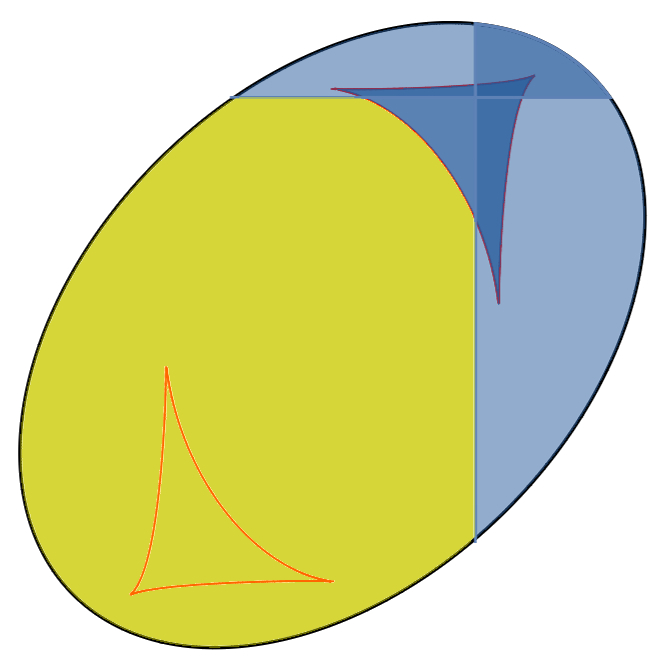
\includegraphics[width=6cm]{RA_example_2.jpg} \ }
\caption{Possible and prohibits cosine values}
\end{figure} 

Figure 4 shows a typical image created by Mathematica code\footnote{Available from the author upon request.} for particlar values of the parameters $\angle A$, $\angle B$, $\angle C$ and $\alpha$. It plots $c_2 \, (=\cos\beta)$ against $c_3 \, (=\cos\gamma)$. The interior of the large ellipse is where Rule 1 is satisfied (equivalently, where $H > 0$), and the focus here is on this region. The blue subregion (darker subregion in the grayscale rendering) consists of points whose coordinates $(c_2, c_3)$ are possible. These are determined by carefully generating possible P3P setups. This is done using the extension of ``Sullivan's method" discussed in \cite{R2}, and this does not involve the claims in Conjecture 1. Darker shades of blue reflect multiple ways to obtain the allowable $(c_2, c_3)$ pair, and this is of no importance here. 

The yellowish subregion (lightest subregion in a grayscale rendering) shows the points $(c_2, c_3)$ for which Item 1 in Conjecture 1 is satisfied, but at least one of the other item is not satisfied. Together, the blue subregion and the yellowish subregion partition the region inside of an ellipse. It was carefully checked that these two subregions do not overlap. This suggests that Conjecture 1 holds for the prescibed values of $\angle A$, $\angle B$, $\angle C$ and $\alpha$. 

The figure also shows a (red) curve, which is where $D = 0$ inside the ellipse. Notice that part of this curve serves as a boundary between the blue and yellow subregions, highlighting the importance of the quantity $D$. Many images similar to Figure 4 have been produced, all supporting Conjecture 1. 


\section{Conclusion} 

Conjecture 1 provides fairly simple criteria that appear to be required in order for a tetrahedron $\Delta ABCP$ to exist with prescribed values for $\angle A$ (= $\angle CAB$), $\angle B$ (= $\angle ABC$), $\angle C$ (= $\angle BCA$), $\alpha$ (= $\angle BPC$),  $\beta$ (= $\angle CPA$) and $\gamma$ (= $\angle APB$). Most of these claims concerning necessity have been proved in this paper. Conjecture 1 can be regarded as criteria for the Perspective 3-Point Problem to have a real solution. Experimental evidence from a couple C++ programs and several Mathematica notebooks lends substantial support to the conjecture. This is based on the assumption that the triangle $\Delta ABC$ is acute. 

Work is underway on extending the results to the case where $\Delta ABC$ is an obtuse, rather than acute, triangle. Already it is clear from the evidence that this is reasonable, and that probably all that is required is some sort of tweaking of the formulas in Conjecture 1. However, no claim concerning the obtuse triangle case is being advanced in this paper, beyond the fact that the ``sphere-based rules" (Items 1, 2 and 3 in Conjecture 1) are also valid for this case too. Using C++ and Mathematica programs, one can plainly observe that some sort of alteration of the deltoid-based rules (Items 6 and 7 in Conjecture 1) is needed. The importance of the quantity $D$ here too is unmistakable.   \\

\section{Appendix}

The ``algebraic proof" of Theorem 1 begins with an arbitrary tetrahedron $\Delta ABCP$. Consider the system of evident equations and inequalities involving the interior angles of all four faces the tetradedron. There are twelve such angles, six of which are $\angle A = \angle CAB$, $\angle B = \angle ABC$, $\angle C = \angle BCA$, $\alpha = BPC$, $\beta = \angle CPA$ and $\gamma = \angle APB$. The other six will be denoted $\alpha' = \angle PCB$, $\beta' = \angle PAC$, $\gamma\,' = \angle PBA$, $\alpha'' = \angle CBP$, $\beta'' = \angle ACP$ and $\gamma\,'' = \angle BAP$. 
All the angles are between 0 and $\pi$. The sum of the three angles at a particular vertex cannot exceed $2\pi$. Of course, the sum of the three angles for a particular face must equal $\pi$. 

To be more specific, we begin with this system of equations and inequalities: $\angle A + \angle B +\angle C = \pi$, $\alpha + \alpha' + \alpha'' = \pi$, $\beta + \beta' + \beta'' = \pi$, $\gamma + \gamma\,' + \gamma\,'' = \pi$, $\angle A > 0$, $\angle B > 0$, $\angle C > 0$, $\alpha > 0$, $\beta > 0$, $\gamma > 0$, $\alpha' > 0$, $\beta' > 0$, $\gamma\,' > 0$, $\alpha'' > 0$, $\beta'' > 0$, $\gamma\,'' > 0$, $\alpha + \beta + \gamma < 2\pi$, $\alpha < \beta + \gamma$, $\beta < \gamma + \alpha$, $\gamma < \alpha + \beta$, $\angle A + \beta' + \gamma\,'' < 2\pi$, $\angle A < \beta' + \gamma\,''$, $\beta' < \gamma\,'' + \angle A$, $\gamma\,'' < \angle A + \beta'$, 
$\alpha'' + \angle B + \gamma\,' < 2\pi$, $\alpha'' < \angle B + \gamma\,'$, $\angle B < \gamma\,' + \alpha''$, $\gamma\,' < \alpha'' + \angle B$, $\alpha' + \beta'' + \angle C < 2\pi$, $\alpha' < \beta'' + \angle C$, $\beta'' < \angle C + \alpha'$, $\angle C < \alpha' + \beta''$. 

This system can easily be reduced to a system of strict inequalities involving eight unknowns, by substituting $\pi - \angle A - \angle B$ for $\angle C$, $\pi - \alpha - \alpha'$ for $\alpha''$, $\pi - \beta - \beta'$ for $\beta''$, and $\pi - \gamma - \gamma\,'$ for $\gamma\,''$. Using Fourier-Motzkin elimination \cite{DE}, one can now eliminate the three primed variables, leaving a system of strict inequalities in $\angle A$, $\angle B$, $\alpha$, $\beta$ and $\gamma$. The result is a system consisting of inequalities that are trivial or sphere-based rules (expressed without using $\angle C$). The following Mathematica code\footnote{Available at\\ {\small \tt https://github.com/mqrieck\\/tetrahedron\_test.cpp/Eliminate.nb}} proceeds along these lines to produce such a system. The only resulting non-trivial rules are essentially Items 1 and 2 in Conjecture 1; Item 3 follows from these, as indicated by Proposition 1. \\ 

{\scriptsize
\begin{alltt} 
(* 
   Displays the inequalities represented by a matrix.
   Each row holds the coefficients of \(\pi\), \(\angle\)\(A\), \(\angle\)\(B\), \(\alpha\), \(\beta\),
    \(\gamma\), \(\alpha'\), \(\beta'\) and \(\gamma\,'\), for a strictly positive quantity. 
*)
showIneqs[mat_] := Module[ \{i, j, len, abs, s\}, 
  len = Length[mat];
  For[i=1, i<=len, i++,
    s = ""; 
    For[j=1, j<=9, j++,
      If[mat[[i]][[j]]>0, s = s <> "+"];
      If[mat[[i]][[j]]<0, s = s <> "-"];
      abs=Abs[mat[[i]][[j]]];
      If[Not[IntegerQ[abs]], abs=N[abs]];
      If[abs!=0 && abs!=1, s=s <>ToString[abs]]; 
      If[abs!=0, 
        If[j==1, s = s <> "\(\pi\)"];
        If[j==2, s = s <> "A"];
        If[j==3, s = s <> "B"];
        If[j==4, s = s <> "\(\alpha\)"];
        If[j==5, s = s <> "\(\beta\)"];
        If[j==6, s = s <> "\(\gamma\)"];
        If[j==7, s = s <> "\(\alpha'\)"];
        If[j==8, s = s <> "\(\beta'\)"];
        If[j==9, s = s <> "\(\gamma\,'\)"]
      ]
    ];
    Print[ToString[i] <> ": " <> s]
  ]
]

(* example *)
showIneqs[\{\{3, 0, 1, -2, 1/4, 0, 0, -5, -1/2\}\}] 
(* +3\(\pi\)+B-2\(\alpha\)+0.25\(\beta\)-5\(\beta'\)-0.5\(\gamma\,'\) *)

(* 
  Assuming all entries in specified column are -1, 0 or 1, 
  eliminate the corresponding variable (Fourier-Motzkin)
  to produce a new matrix.
*)
elim[mat_,index_]:= Module[ \{i, j, len, newmat\},
  newmat=\{\};
  len = Length[mat] ;
  For[i=1, i<=len, i++, 
    If[mat[[i]][[index]] == 0, AppendTo[newmat,mat[[i]]]]];
    For[i=1, i<=len, i++, 
      If[mat[[i]][[index]] == 1, 
      For[j=1, j<=len, j++, 
        If[mat[[j]][[index]] == -1, 
          AppendTo[newmat,mat[[i]]+mat[[j]]]
        ]
      ]
    ]  
  ];
  newmat
]

(*
  Scale each row of the matrix so that the entry in the 
  specified column is either -1, 0 or 1.
*)
normal[ mat_, index_] := Module[ \{i, j, len, newmat\}, 
  newmat=\{\};
  len = Length[mat]; 
  For[i=1, i <= len, i++, 
    If[mat[[i]][[index]] == 0, 
      AppendTo[newmat, mat[[i]]], 
      AppendTo[newmat, mat[[i]]/Abs[mat[[i]][[index]]]]
    ]
  ];
  newmat
]

(* 
  Scale each row of integers so that its GCD is 1;  
  Also, remove duplicate rows. 
*)
clean[mat_] := Module[ \{i, j, len, len2, newmat\}, 
  newmat = \{\}; 
  len = Length[mat]; 
  For[i=1, i<=len, i++,
    If[And @@ IntegerQ /@ mat[[i]], 
      AppendTo[newmat, mat[[i]] / GCD @@ mat[[i]]], 
      AppendTo[newmat, mat[[i]] ]
    ]; 
  ];
  newmat = DeleteDuplicates[newmat]; 
  newmat
]

(* 
  Used to convert final matrix to integers only,
  and to remove repeated rows.
*)
tweak[mat_] := Module[ \{i, j, len, len2, newmat\} , 
  newmat = \{\}; 
  len = Length[mat]; 
  For[i=1, i<=len, i++,
    If[And @@ IntegerQ /@ mat[[i]], 
      AppendTo[newmat, mat[[i]]], 
      AppendTo[newmat, 2 mat[[i]] ]
    ]; 
  ];
  newmat = DeleteDuplicates[newmat]; 
  newmat
]

(*
  Find and remove redundant inequality rows from a 
  matrix, using linear programming.
*)
reduce[mat_, startindex_] := Module[ 
  \{i, len, len0, newmat, lower, vector\}, 
  newmat = mat;
  len0 = Length[mat];   
  For[ i = len0, i >= startindex, i--, 
    len = Length[newmat]; 
    lower = ConstantArray[0, len];
    lower[[i]]= -1;
    vector = LinearProgramming[newmat[[i]], newmat, lower, 
      \{\{1,1\}, \{0,1\}, \{0,1\}, \{0,1\}, \{0,1\}, \{0,1\}, \{0,1\},
      \{0,1\}, \{0,1\}\}];
    If[vector. newmat[[i]] == 0, newmat = Delete[newmat,i]]
  ];
  newmat
]

(* 
  Matrix describing tetrahedron angles inequalities
*)
M1 = \{
  \{  1,  0,  0,  0,  0,  0,  0,  0,  0 \}, 
  \{  0,  1,  0,  0,  0,  0,  0,  0,  0 \}, 
  \{  0,  0,  1,  0,  0,  0,  0,  0,  0 \}, 
  \{  0,  0,  0,  1,  0,  0,  0,  0,  0 \}, 
  \{  0,  0,  0,  0,  1,  0,  0,  0,  0 \}, 
  \{  0,  0,  0,  0,  0,  1,  0,  0,  0 \}, 
  \{  0,  0,  0,  0,  0,  0,  1,  0,  0 \}, 
  \{  0,  0,  0,  0,  0,  0,  0,  1,  0 \}, 
  \{  0,  0,  0,  0,  0,  0,  0,  0,  1 \}, 
  \{  1, -1, -1,  0,  0,  0,  0,  0,  0 \}, 
  \{  1,  0,  0, -1,  0,  0, -1,  0,  0 \}, 
  \{  1,  0,  0,  0, -1,  0,  0, -1,  0 \}, 
  \{  1,  0,  0,  0,  0, -1,  0,  0, -1 \}, 
  \{  2,  0,  0, -1, -1, -1,  0,  0,  0 \}, 
  \{  0,  0,  0, -1,  1,  1,  0,  0,  0 \}, 
  \{  0,  0,  0,  1, -1,  1,  0,  0,  0 \}, 
  \{  0,  0,  0,  1,  1, -1,  0,  0,  0 \}, 
  \{  1, -1,  0,  0,  0,  1,  0, -1,  1 \}, 
  \{  1, -1,  0,  0,  0, -1,  0,  1, -1 \}, 
  \{  1,  1,  0,  0,  0, -1,  0, -1, -1 \}, 
  \{ -1,  1,  0,  0,  0,  1,  0,  1,  1 \}, 
  \{  1,  0, -1,  1,  0,  0,  1,  0, -1 \}, 
  \{  1,  0, -1, -1,  0,  0, -1,  0,  1 \},
  \{  1,  0,  1, -1,  0,  0, -1,  0, -1 \}, 
  \{ -1,  0,  1,  1,  0,  0,  1,  0,  1 \}, 
  \{  0,  1,  1,  0,  1,  0, -1,  1,  0 \}, 
  \{  0,  1,  1,  0, -1,  0,  1, -1,  0 \}, 
  \{  2, -1, -1,  0, -1,  0, -1, -1,  0 \}, 
  \{  0, -1, -1,  0,  1,  0,  1,  1,  0 \}
\} ;
showIneqs[M1] 

1: +\(\pi\)
2: +A
3: +B
4: +\(\alpha\)
5: +\(\beta\)
6: +\(\gamma\)
7: +\(\alpha\)'
8: +\(\beta\)'
9: +\(\gamma\)'
10: +\(\pi\)-A-B
11: +\(\pi\)-\(\alpha\)-\(\alpha\)'
12: +\(\pi\)-\(\beta\)-\(\beta\)'
13: +\(\pi\)-\(\gamma\)-\(\gamma\)'
14: +2\(\pi\)-\(\alpha\)-\(\beta\)-\(\gamma\)
15: -\(\alpha\)+\(\beta\)+\(\gamma\)
16: +\(\alpha\)-\(\beta\)+\(\gamma\)
17: +\(\alpha\)+\(\beta\)-\(\gamma\)
18: +\(\pi\)-A+\(\gamma\)-\(\beta\)'+\(\gamma\)'
19: +\(\pi\)-A-\(\gamma\)+\(\beta\)'-\(\gamma\)'
20: +\(\pi\)+A-\(\gamma\)-\(\beta\)'-\(\gamma\)'
21: -\(\pi\)+A+\(\gamma\)+\(\beta\)'+\(\gamma\)'
22: +\(\pi\)-B+\(\alpha\)+\(\alpha\)'-\(\gamma\)'
23: +\(\pi\)-B-\(\alpha\)-\(\alpha\)'+\(\gamma\)'
24: +\(\pi\)+B-\(\alpha\)-\(\alpha\)'-\(\gamma\)'
25: -\(\pi\)+B+\(\alpha\)+\(\alpha\)'+\(\gamma\)'
26: +A+B+\(\beta\)-\(\alpha\)'+\(\beta\)'
27: +A+B-\(\beta\)+\(\alpha\)'-\(\beta\)'
28: +2\(\pi\)-A-B-\(\beta\)-\(\alpha\)'-\(\beta\)'
29: -A-B+\(\beta\)+\(\alpha\)'+\(\beta\)'

(* Eliminate \(\gamma\,'\) and normalize for \(\beta'\) *)
showIneqs[ M2 = clean[normal[elim[M1,9],8]] ] 

1: +\(\pi\)
2: +A
3: +B
4: +\(\alpha\)
5: +\(\beta\)
6: +\(\gamma\)
7: +\(\alpha\)'
8: +\(\beta\)'
9: +\(\pi\)-A-B
10: +\(\pi\)-\(\alpha\)-\(\alpha\)'
11: +\(\pi\)-\(\beta\)-\(\beta\)'
12: +2\(\pi\)-\(\alpha\)-\(\beta\)-\(\gamma\)
13: -\(\alpha\)+\(\beta\)+\(\gamma\)
14: +\(\alpha\)-\(\beta\)+\(\gamma\)
15: +\(\alpha\)+\(\beta\)-\(\gamma\)
16: +A+B+\(\beta\)-\(\alpha\)'+\(\beta\)'
17: +A+B-\(\beta\)+\(\alpha\)'-\(\beta\)'
18: +2\(\pi\)-A-B-\(\beta\)-\(\alpha\)'-\(\beta\)'
19: -A-B+\(\beta\)+\(\alpha\)'+\(\beta\)'
20: +\(\pi\)-\(\gamma\)
21: +\(\pi\)-A-\(\gamma\)+\(\beta\)'
22: +\(\pi\)+A-\(\gamma\)-\(\beta\)'
23: +\(\pi\)-B+\(\alpha\)+\(\alpha\)'
24: +\(\pi\)+B-\(\alpha\)-\(\alpha\)'
25: +2\(\pi\)-A-\(\beta\)'
26: +\(\pi\)-A
27: +\(\pi\)-\(\beta\)'
28: +2\(\pi\)-A-B+\(\alpha\)+\(\gamma\)+\(\alpha\)'-\(\beta\)'
29: +2\(\pi\)-A+B-\(\alpha\)+\(\gamma\)-\(\alpha\)'-\(\beta\)'
30: +A+\(\beta\)'
31: +A-B+\(\alpha\)+\(\gamma\)+\(\alpha\)'+\(\beta\)'
32: +A+B-\(\alpha\)+\(\gamma\)-\(\alpha\)'+\(\beta\)'
33: +2\(\pi\)-B-\(\alpha\)-\(\gamma\)-\(\alpha\)'
34: +2\(\pi\)-A-B-\(\alpha\)-\(\gamma\)-\(\alpha\)'+\(\beta\)'
35: +2\(\pi\)+A-B-\(\alpha\)-\(\gamma\)-\(\alpha\)'-\(\beta\)'
36: +\(\pi\)-B
37: +B+\(\alpha\)-\(\gamma\)+\(\alpha\)'
38: -A+B+\(\alpha\)-\(\gamma\)+\(\alpha\)'+\(\beta\)'
39: +A+B+\(\alpha\)-\(\gamma\)+\(\alpha\)'-\(\beta\)'
40: +\(\alpha\)+\(\alpha\)'

(* Delete redundant inequalities *) 
showIneqs[ M3 = reduce[M2, 9] ]

1: +\(\pi\)
2: +A
3: +B
4: +\(\alpha\)
5: +\(\beta\)
6: +\(\gamma\)
7: +\(\alpha\)'
8: +\(\beta\)'
9: +\(\pi\)-\(\alpha\)-\(\alpha\)'
10: -\(\alpha\)+\(\beta\)+\(\gamma\)
11: +\(\alpha\)-\(\beta\)+\(\gamma\)
12: +\(\alpha\)+\(\beta\)-\(\gamma\)
13: +A+B-\(\beta\)+\(\alpha\)'-\(\beta\)'
14: +2\(\pi\)-A-B-\(\beta\)-\(\alpha\)'-\(\beta\)'
15: -A-B+\(\beta\)+\(\alpha\)'+\(\beta\)'
16: +A+B-\(\alpha\)+\(\gamma\)-\(\alpha\)'+\(\beta\)'
17: +2\(\pi\)-A-B-\(\alpha\)-\(\gamma\)-\(\alpha\)'+\(\beta\)'
18: +2\(\pi\)+A-B-\(\alpha\)-\(\gamma\)-\(\alpha\)'-\(\beta\)'
19: -A+B+\(\alpha\)-\(\gamma\)+\(\alpha\)'+\(\beta\)'

(* Eliminate \(\beta'\) and normalize for \(\alpha'\) *)
showIneqs[ M4 = clean[normal[elim[M3, 8], 7]] ] 

1: +\(\pi\)
2: +A
3: +B
4: +\(\alpha\)
5: +\(\beta\)
6: +\(\gamma\)
7: +\(\alpha\)'
8: +\(\pi\)-\(\alpha\)-\(\alpha\)'
9: -\(\alpha\)+\(\beta\)+\(\gamma\)
10: +\(\alpha\)-\(\beta\)+\(\gamma\)
11: +\(\alpha\)+\(\beta\)-\(\gamma\)
12: +A+B-\(\beta\)+\(\alpha\)'
13: +2\(\pi\)-A-B-\(\beta\)-\(\alpha\)'
14: +2\(\pi\)+A-B-\(\alpha\)-\(\gamma\)-\(\alpha\)'
15: +\(\pi\)-A-B
16: +2\(\pi\)-2B-\(\alpha\)+\(\beta\)-\(\gamma\)
17: +2A+2B-\(\alpha\)-\(\beta\)+\(\gamma\)
18: +\(\pi\)-0.5\(\alpha\)-0.5\(\beta\)+0.5\(\gamma\)-\(\alpha\)'
19: +\(\pi\)+A-\(\alpha\)-\(\alpha\)'
20: +2\(\pi\)-\(\alpha\)-\(\beta\)-\(\gamma\)
21: +2\(\pi\)-A-B-0.5\(\alpha\)-0.5\(\beta\)-0.5\(\gamma\)-\(\alpha\)'
22: +2\(\pi\)-B-\(\alpha\)-\(\gamma\)-\(\alpha\)'
23: +B+0.5\(\alpha\)-0.5\(\beta\)-0.5\(\gamma\)+\(\alpha\)'
24: +2\(\pi\)-2A+\(\alpha\)-\(\beta\)-\(\gamma\)
25: +\(\pi\)-\(\gamma\)

(* Delete redundant inequalities *) 
showIneqs[ M5 = reduce[M4, 8] ]

1: +\(\pi\)
2: +A
3: +B
4: +\(\alpha\)
5: +\(\beta\)
6: +\(\gamma\)
7: +\(\alpha\)'
8: +\(\pi\)-\(\alpha\)-\(\alpha\)'
9: -\(\alpha\)+\(\beta\)+\(\gamma\)
10: +\(\alpha\)-\(\beta\)+\(\gamma\)
11: +\(\alpha\)+\(\beta\)-\(\gamma\)
12: +A+B-\(\beta\)+\(\alpha\)'
13: +\(\pi\)-A-B
14: +2\(\pi\)-2B-\(\alpha\)+\(\beta\)-\(\gamma\)
15: +2A+2B-\(\alpha\)-\(\beta\)+\(\gamma\)
16: +2\(\pi\)-\(\alpha\)-\(\beta\)-\(\gamma\)
17: +2\(\pi\)-A-B-0.5\(\alpha\)-0.5\(\beta\)-0.5\(\gamma\)-\(\alpha\)'
18: +2\(\pi\)-B-\(\alpha\)-\(\gamma\)-\(\alpha\)'
19: +B+0.5\(\alpha\)-0.5\(\beta\)-0.5\(\gamma\)+\(\alpha\)'
20: +2\(\pi\)-2A+\(\alpha\)-\(\beta\)-\(\gamma\)

(* Eliminate \(\alpha'\) *)
showIneqs[ M6 = tweak[clean[elim[M5, 7]]] ] 

1: +\(\pi\)
2: +A
3: +B
4: +\(\alpha\)
5: +\(\beta\)
6: +\(\gamma\)
7: -\(\alpha\)+\(\beta\)+\(\gamma\)
8: +\(\alpha\)-\(\beta\)+\(\gamma\)
9: +\(\alpha\)+\(\beta\)-\(\gamma\)
10: +\(\pi\)-A-B
11: +2\(\pi\)-2B-\(\alpha\)+\(\beta\)-\(\gamma\)
12: +2A+2B-\(\alpha\)-\(\beta\)+\(\gamma\)
13: +2\(\pi\)-\(\alpha\)-\(\beta\)-\(\gamma\)
14: +2\(\pi\)-2A+\(\alpha\)-\(\beta\)-\(\gamma\)
15: +\(\pi\)-\(\alpha\)
16: +4\(\pi\)-2A-2B-\(\alpha\)-\(\beta\)-\(\gamma\)
17: +2\(\pi\)-B-\(\alpha\)-\(\gamma\)
18: +\(\pi\)+A+B-\(\alpha\)-\(\beta\)
19: +4\(\pi\)-\(\alpha\)-3\(\beta\)-\(\gamma\)
20: +2\(\pi\)+A-\(\alpha\)-\(\beta\)-\(\gamma\)
21: +2\(\pi\)+2B-\(\alpha\)-\(\beta\)-\(\gamma\)
22: +2\(\pi\)-A-\(\beta\)-\(\gamma\)
23: +4\(\pi\)-\(\alpha\)-\(\beta\)-3\(\gamma\)

(* Delete redundant inequalities *) 
showIneqs[ M7 = reduce[M6, 7] ]

1: +\(\pi\)
2: +A
3: +B
4: +\(\alpha\)
5: +\(\beta\)
6: +\(\gamma\)
7: -\(\alpha\)+\(\beta\)+\(\gamma\)
8: +\(\alpha\)-\(\beta\)+\(\gamma\)
9: +\(\alpha\)+\(\beta\)-\(\gamma\)
10: +\(\pi\)-A-B
11: +2\(\pi\)-2B-\(\alpha\)+\(\beta\)-\(\gamma\)
12: +2A+2B-\(\alpha\)-\(\beta\)+\(\gamma\)
13: +2\(\pi\)-\(\alpha\)-\(\beta\)-\(\gamma\)
14: +2\(\pi\)-2A+\(\alpha\)-\(\beta\)-\(\gamma\)

\end{alltt}  
}

\renewcommand{\baselinestretch}{0.98}

\bibliographystyle{apalike}
{\small

\begin{thebibliography}{}

\bibitem[Dantzig-Eaves, 1973]{DE}
Dantzig, G. B., Eaves, B. C. (1973)
\newblock Fourier-Motzkin elimination and its dual.
\newblock {\em J. Combinatorial Theory, Series A}, 14(3): 288--297. 

\bibitem[Faug\`ere et~al., 2008]{FMRE}
Faug\`ere, J.-C., Moroz, G., Rouillier, F., and El-Din, M.~S. (2008).
\newblock Classification of the perspective-three-point problem, discriminant variety and real solving polynomial systems of inequalities.
\newblock In {\em ISSAC'08, 21st Int. Symp. Symbolic and Algebraic Computation}, 79--86.

\bibitem[Gao et~al., 2003]{GHTC}
Gao, X.-S., Hou, X.-R., Tang, J., and Cheng, H.-F. (2003).
\newblock Complete solution classification for the perspective-three-point problem.
\newblock {\em IEEE Trans. Pattern Analysis and Machine Intelligence}, 25(8): 930--943.

\bibitem[Grunert, 1841]{G}
Grunert, J.~A. (1841).
\newblock Das pothenotische problem in erweiterter gestalt nebst {\"u}ber seine anwendungen in der geod{\"a}sie.
\newblock In {\em Grunerts Archiv f{\"u}r Mathematik und Physik}, 1: 238--248.

\bibitem[Haralick et~al., 1994]{HLON}
Haralick, R.~M., Lee, C.-N., Ottenberg, K., and N{\"o}lle, N. (1994).
\newblock Review and analysis of solutions of the three point perspective pose estimation problem.
\newblock {\em J. Computer Vision}, 13(3): 331--356.

\bibitem[Rieck, 2018]{R1}
Rieck, M.~Q. (2018).
\newblock On the discriminant of Grunert's system of algebraic equations and related topics.
\newblock {\em J. Mathematical Imaging and Vision}, 60(5):  737-762.

\bibitem[Rieck, 2023, 1]{R2}
Rieck, M.~Q. (2023, 1).
\newblock Related problems in spherical and solid geometry.  
\newblock {\em Int. J. Geometry}, 12(2): 117--124. 

\bibitem[Rieck, 2023, 2]{R3}
Rieck, M.~Q. (2023, 2).
\newblock Understanding the deltoid phenomenon in the perspective 3-point problem.  
\newblock {\em Posted preprint:} https://www.techrxiv.org/articles/preprint/\\Understanding\_the\_Deltoid\_Phenomenon\_in\_the\_\\Perspective\_3-Point\_Problem/21781268.

\bibitem[Rieck, under review]{R4}
Rieck, M.~Q.
\newblock Angular properties of a tetrahedron with an acute triangular base.
\newblock {\em Annali di Matematica Pura et Applicata}, under review.

\bibitem[Rieck-Wang, 2021]{RW}
Rieck, M.~Q., and Wang, B. (2021). 
\newblock Locating Perspective Three-Point Problem Solutions in Spatial Regions.
\newblock {\em J. Mathematical Imaging and Vision}, 63(8): 953-973.

\end{thebibliography} }


\end{document}


